\begin{abox}
	Net-June-2020
	\end{abox}
\section{PART A}
\begin{enumerate}
	\item A couple lives in a house with their sons and daughters and no one else. The couple has four sons and each of the sons has exactly two sisters. How many persons live in that house?
	 \begin{tasks}(4)
		\task[\textbf{a.}]8
		\task[\textbf{b.}]10
		\task[\textbf{c.}]12
		\task[\textbf{d.}] 14
	\end{tasks}
\begin{answer}
 A couple has 2 persons. There are four sons and each son has two sisters. Hence total number of persons $=2+4+2=8$\\
So the correct answer is \textbf{Option (a)}
\end{answer}
\item A bank pays interest to its depositors compounded yearly. If a deposit becomes Rs. $54,000 /-$ at the end of $3^{\text {rd }}$ year and Rs. $64,800 /-$ at the end of $6^{\text {th }}$ year, what is the principal invested in the deposit?
 \begin{tasks}(4)
	\task[\textbf{a.}]40,000
	\task[\textbf{b.}]42,000
	\task[\textbf{c.}]45,000
	\task[\textbf{d.}] 48,000
\end{tasks}
\begin{answer}
	\begin{align}
\text{	Let the principal }&\text{invested be $P$. Then from the question}\notag\\
	54000&=P\left(1+\frac{r}{100}\right)^{3} \label{20-1}\\
	64800&=P\left(1+\frac{r}{100}\right)^{6}\label{20-2}\\
\text{	Squaring equation }&\text{(\ref{20-1}) and dividing by equation (\ref{20-2}) gives}\notag\\
	\frac{P^{2}}{P}&=\frac{(54000)^{2}}{64800} \Rightarrow P=45000 \notag
	\end{align}
	So the correct answer is \textbf{Option (c)}
\end{answer}
\item In the following $\triangle A B C, A B=7 \mathrm{~cm}, B C=15 \mathrm{~cm}$ and $A C=12 \mathrm{~cm} . D$ is a point on $B C$ such that $\triangle A D C$ and $\triangle A B C$ are similar. Then $A D($ in $\mathrm{cm})=$	
\begin{figure}[H]
	\centering
	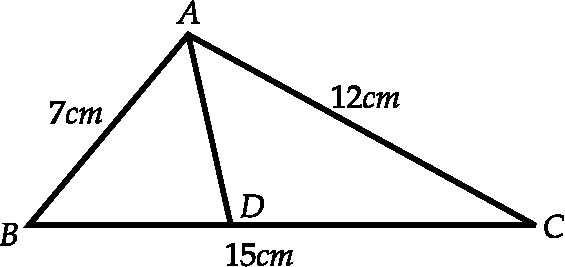
\includegraphics[height=2.5cm,width=5cm]{Net-June-20-1}
\end{figure}	
 \begin{tasks}(4)
	\task[\textbf{a.}]$5.6$
	\task[\textbf{b.}]$5.8$
	\task[\textbf{c.}] $6.1$
	\task[\textbf{d.}]$6.4$ 
\end{tasks}
\begin{answer}
	\begin{align*}
\text{The correct wording }&\text{of the question should be $\triangle A D C$ is similar to $\triangle B A C$.}\\
	\text{From the similarity }&\text{condition we can write}\\
	\frac{A D}{A C}&=\frac{A B}{B C} \Rightarrow A D=\frac{A B}{B C} \times A C \\
	\Rightarrow A D&=\frac{7}{15} \times 12=5.6
	\end{align*}
	So the correct answer is \textbf{Option (a)}
\end{answer}
\item Ten glass vases were to be packed one each in 10 boxes marked "Glass". Twelve brass vases were to be packed one each in 12 boxes marked "Brass". Four vases and boxes got mixed up. A customer orders 1 glass and 1 brass vase and is sent appropriately marked boxes. The chance that the customer does not get the ordered vases in correctly marked boxes is
 \begin{tasks}(4)
	\task[\textbf{a.}]$4 / 5$
	\task[\textbf{b.}]$5 / 6$
	\task[\textbf{c.}]$2 / 3$
	\task[\textbf{d.}] $1 / 3$
\end{tasks}
\begin{answer}
	 According to wording of question, total four vases and boxes are mixed up. This is possible when 2 Glass boxes are mixed up and two Brass boxes are mixed up.
	 \begin{figure}[H]
	 	\centering
	 	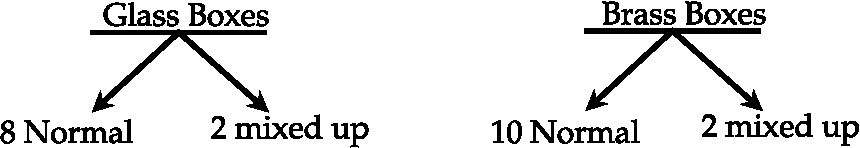
\includegraphics[height=1.3cm,width=7.5cm]{Net-June-20-2}
	 \end{figure}
	\begin{align*}
\text{	Total number of ways }&\text{of not drawing 1 glass box and 1 brass box correctly}\\
	&=8 \times 2+2 \times 10+2 \times 2=16+20+4=40\\
	\text{Total number of ways }&\text{of drawing 1 glass box and 1 brass box correctly}\\
	&=10 \times 12=120\\
\text{	Required probability }&=\frac{40}{120}=\frac{1}{3}
	\end{align*}
		So the correct answer is \textbf{Option (d)}
\end{answer}
\item Anwara, Bharati, Colin and Tarun commute by different modes of transport namely, Cycle (C), Autorickshaw (A), Bus (B) and Train (T). The initials of the mode of transport and the name of the person match in exactly two cases. If Tarun travels by Train, and Colin rides neither an Autorickshaw nor a Bus, then 
 \begin{tasks}(2)
	\task[\textbf{a.}]Anwara rides an Autorikshaw
	\task[\textbf{b.}]Anwara rides a Bus
	\task[\textbf{c.}]Bharati rides a Bus
	\task[\textbf{d.}] Bharati rides a Cycle
\end{tasks}
\begin{answer}
	 Tarun travels by Train. Colin rides neither an Autorickshaw nor a Bus hence Colin definitely travels by Cycle. Here we see that for both Tarun and Colin have their initials match with their mode of transports. Since, the initials of only two persons can match with their mode of transports, hence Anawara must ride a Bus and Bharati must ride an Autorickshaw.\\
	So the correct answer is \textbf{Option (b)}
\end{answer}
\item Rice production in six states $A, B, C, D, E$ and $F$ in two consecutive years are shown in the diagram in linear scale
\begin{figure}[H]
	\centering
	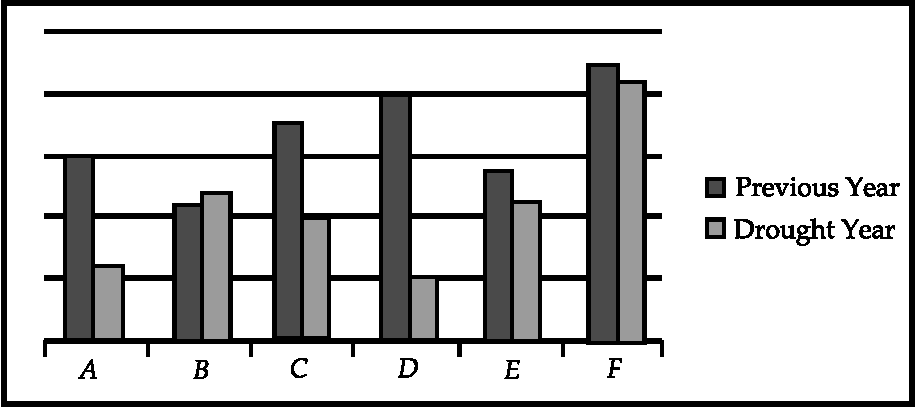
\includegraphics[height=4cm,width=8.3cm]{Net-June-20-3}
\end{figure}
Among the states that saw a fall in production in the drought year, the maximum and minimum relative fall was, respectively, in states,
 \begin{tasks}(4)
	\task[\textbf{a.}]$D$ and $F$
	\task[\textbf{b.}]$C$ and $B$
	\task[\textbf{c.}]$C$ and $E$
	\task[\textbf{d.}] $D$ and $A$
\end{tasks}
\begin{answer}
	\begin{align*}
	\text { Relative fall }&=\frac{\text { Fall }}{\text { Previous output }}\\
	\text{Using this relation we see}&\text{ that maximum relative fall was in state $D$ and minimum relative fall was in state $F$.}
	\end{align*}
		So the correct answer is \textbf{Option (a)}
\end{answer}
\item  Based on the table, what is the maximum number of diamonds one can buy for Rs. 10 lakh?\\\\
\begin{tabular}{|c|c|c|}
	\hline Size (in carat) & Rate (Rs. Lakh per carat) & Number in stock \\
	\hline $0.25$ & 1 & 20 \\
	\hline $0.5$ & 2 & 10 \\
	\hline 1 & 4 & 5 \\
	\hline 2 & 8 & 1 \\
	\hline
\end{tabular}\\\\
 \begin{tasks}(4)
	\task[\textbf{a.}]20
	\task[\textbf{b.}]25
	\task[\textbf{c.}]30
	\task[\textbf{d.}] 36
\end{tasks}
\begin{answer}
	\begin{align*}
	\intertext{In order to buy maximum number of diamonds, we must start with diamond size with cheapest rate then next cheapest and so on.}
	&\text{All 20 diamonds with carat size $0.25$ can be purchased.}\\
	&\text{This is because $20 \times 0.25 \times 2=5$ lakh}\\
   &\text{	Only 5 diamonds of $0.5$ carat size can be purchased}\\
&\text{	This is because}\\
	&5 \times 0.5 \times 2=5 \text { lakh }\\
	&\text{Now all money has been exhausted and no further diamonds can be purchased.}\\
	&\text{Hence required answer $=20+5=25$}
	\end{align*}
			So the correct answer is \textbf{Option (b)}
\end{answer}
\item For a disease, every infected person infects three others on the $5^{\text {th }}$ day and recovers. On an average, men and women are infected in the proportion 4:1. The total number of women who were infected by the end of 35 days, is closest to
 \begin{tasks}(4)
	\task[\textbf{a.}]972
	\task[\textbf{b.}]820
	\task[\textbf{c.}]656
	\task[\textbf{d.}] 502
\end{tasks}
\begin{answer}
	The number of infected persons on the $5,10,15, \ldots \ldots, 35$ days are shown below\\\\
	\renewcommand*{\arraystretch}{1.5}
	\begin{tabular}{|c|c|c|c|c|c|c|}
		\hline Days & 5 & 10 & 15 &\dots &30&35\\
		\hline Infected Persons& 3 & $3^{2}$ & $3^{3}$ &$\dots$& $3^{6}$& $3^{7}$\\
		\hline Infected  women  & $\frac{3}{5}$ & $\frac{3^{2}}{5}$ & $\frac{3^{3}}{5}$&\dots &$\frac{3^{6}}{5}$&$\frac{3^{7}}{5}$\\\hline
	\end{tabular}\\\\
From the above table we see that the total number of infected women who were infected by the end of 35 days is
	\begin{align*}
\frac{3}{5}+\frac{3^{2}}{5}+\frac{3^{3}}{5}+\ldots .+\frac{3^{7}}{5}=\frac{1}{5}\left(3+3^{2}+3^{3}+\ldots .+3^{7}\right)=\frac{3\left(3^{7}-1\right)}{3-1} \approx \frac{3^{8}}{2}=656.1 \approx 656
	\end{align*}
		So the correct answer is \textbf{Option (c)}
\end{answer}
\item The maximum tolerable exposure time for noise is given to be about 8 hours at $85 \mathrm{~dB}$ and 90 seconds at $110 \mathrm{~dB}$. Assuming linear noise tolerance response of the ear, an increase of $3 \mathrm{~dB}$ in noise level in this range would reduce the exposure time by roughly
 \begin{tasks}(4)
	\task[\textbf{a.}]$45 \mathrm{~min}$
	\task[\textbf{b.}]$60 \mathrm{~min}$
	\task[\textbf{c.}]$90 \mathrm{~min}$
	\task[\textbf{d.}]$120 \mathrm{~min}$ 
\end{tasks}
\begin{answer}$\left. \right. $
	\begin{figure}[H]
		\centering
		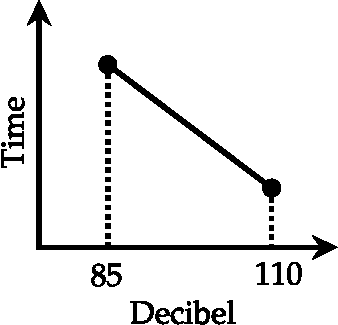
\includegraphics[height=3cm,width=3cm]{Net-June-20-4}
	\end{figure}
	\begin{align*}
	\text{Assuming linearization }&\text{exposure time per unit decibel is}\\
	\frac{480-1.5}{110-85}&=19.14\\
\text{	Hence an increase of }&\text{$3 \mathrm{~dB}$ in noise level would reduce the exposure time by roughly}\\
	19.14 \times 3&=57.42 \approx 60 \mathrm{~min}
	\end{align*}
	So the correct answer is \textbf{Option (b)}
\end{answer}
\item Distance covered by cars, $X$ and $Y$, with time is given below. Assuming constant acceleration for each car, which of the following graphs shows that $X$ had higher acceleration than $Y$ ? \begin{tasks}(2)
	\task[\textbf{a.}]
	\begin{figure}[H]
		\centering
		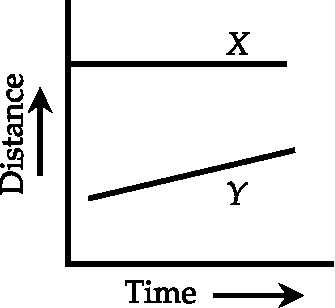
\includegraphics[height=2.5cm,width=2.5cm]{Net-June-20-5}
	\end{figure}
	\task[\textbf{b.}]
		\begin{figure}[H]
		\centering
		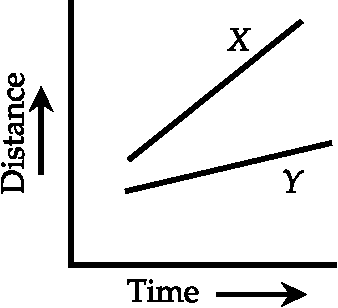
\includegraphics[height=2.5cm,width=2.5cm]{Net-June-20-6}
	\end{figure}
	\task[\textbf{c.}]
		\begin{figure}[H]
		\centering
		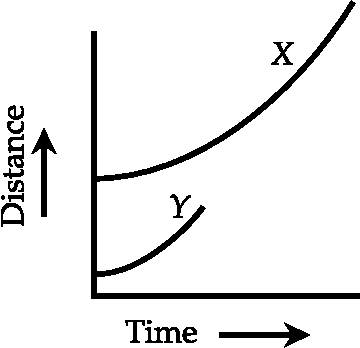
\includegraphics[height=2.5cm,width=2.5cm]{Net-June-20-7}
	\end{figure}
	\task[\textbf{d.}] 
		\begin{figure}[H]
		\centering
		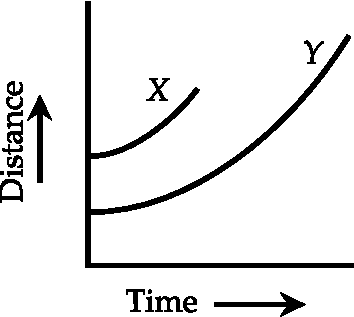
\includegraphics[height=2.5cm,width=2.5cm]{Net-June-20-8}
	\end{figure}
\end{tasks}
\begin{answer}
	The acceleration is given by $a=\frac{d^{2} x}{d t^{2}}$. Thus $a$ is decided by the concavity of distance-time curve. Hence the last graph shows that $X$ has higher acceleration than $Y$.\\
		So the correct answer is \textbf{Option (d)}
\end{answer}
\item  $P Q R S$ is a rectangle inscribed in a quarter circle as shown. The area of shaded region is $24 \mathrm{~cm}^{2}$
and $P Q=6 \mathrm{~cm}$.	
	\begin{figure}[H]
	\centering
	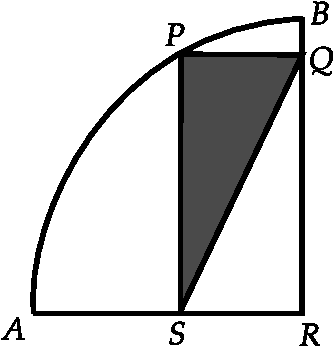
\includegraphics[height=2.5cm,width=2.5cm]{Net-June-20-9}
\end{figure}
The area of the quarter circle is
	 \begin{tasks}(4)
		\task[\textbf{a.}]$36 \pi$
		\task[\textbf{b.}]$25 \pi$
		\task[\textbf{c.}] $13 \pi$
		\task[\textbf{d.}] $48 \pi$
	\end{tasks}
\begin{answer}$\left. \right. $
		\begin{figure}[H]
		\centering
		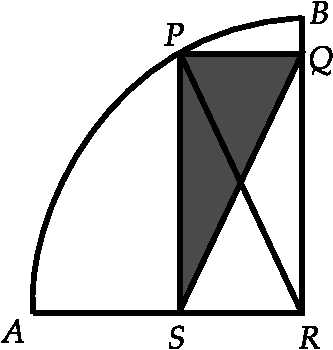
\includegraphics[height=2.5cm,width=2.5cm]{Net-June-20-10}
	\end{figure}
	\begin{align*}
\intertext{ $P Q R S$ is a rectangle, therefore $\angle Q P S=90^{\circ}$ and the triangle $Q P S$ is a right-angled triangle. This gives}
 \frac{1}{2} \times P Q \times P S&=24 \Rightarrow \frac{1}{2} \times 6 \times P S=24 \Rightarrow P S=8\\
	\text{$P R$ is a diagonal of the }&\text{rectangle and it is also the radius of circle.}\\
	P R=\sqrt{(P Q)^{2}+(P S)^{2}}&=\sqrt{6^{2}+8^{2}}=10 \mathrm{~cm}\\
\text{	The area of quarter circle }&\text{(in $\mathrm{cm}^{2}$ ) is $=\frac{\pi(10)^{2}}{4}=25 \pi$}
	\end{align*}
		So the correct answer is \textbf{Option (b)}
\end{answer}
\item Area of the trapezium as shown in the figure, is	
	\begin{figure}[H]
	\centering
	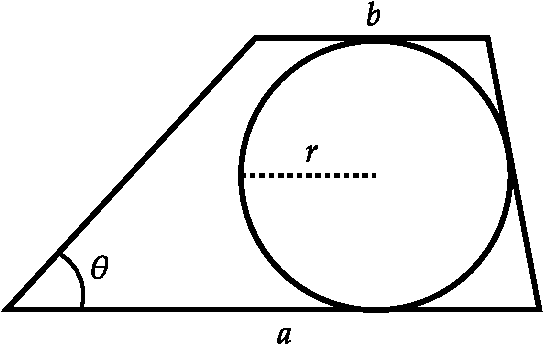
\includegraphics[height=2.5cm,width=4cm]{Net-June-20-11}
\end{figure}
 \begin{tasks}(2)
	\task[\textbf{a.}]$a b+r^{2} \tan \theta$
	\task[\textbf{b.}]$r(a+b) \cos \theta$
	\task[\textbf{c.}]$2 r(a+b)$
	\task[\textbf{d.}] $r(a+b)$
\end{tasks}
\begin{answer}$\left. \right. $
		\begin{figure}[H]
		\centering
		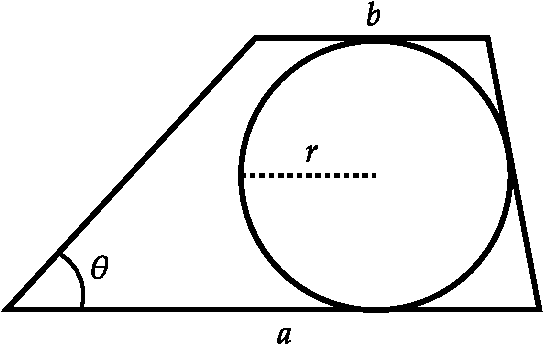
\includegraphics[height=2.5cm,width=4cm]{Net-June-20-11}
	\end{figure}
	\begin{align*}
\text{ The perpendicular distance }&\text{between parallel sides }\\
&=r+r=2 r\\
	\text{Sum of parallel sides }&=a+b\\
\text{	Hence area of trapezium }&=\frac{1}{2} \times(a+b) \times 2 r=r(a+b)
	\end{align*}
		So the correct answer is \textbf{Option (d)}
\end{answer}
\item From an initially full bucket, water is dripping continuously from the bottom. The centre of mass of the bucket with water
 \begin{tasks}(2)
	\task[\textbf{a.}]Remains stationary
	\task[\textbf{b.}]Moves upward all the way
	\task[\textbf{c.}]Moves downward all the way
	\task[\textbf{d.}]Moves downward first and then moves up
\end{tasks}
\begin{answer}
		So the correct answer is \textbf{Option (d)}
\end{answer}
\item Seven persons $A, B, C, D, E, F$ and $G$ are sitting in a row. $E$ and $B$ are sitting adjacent to each other. $F$ is sitting between $D$ and $G$. If $C$ is sitting four places left of $F$, who among the following cannot be sitting at the centre?
 \begin{tasks}(4)
	\task[\textbf{a.}] $G$
	\task[\textbf{b.}] $B$
	\task[\textbf{c.}]$D$
	\task[\textbf{d.}]  $F$
\end{tasks}
\begin{answer}
For any person sitting at the centre, there are exactly three persons to his left and exactly three persons to his right. From the question, there are four or more persons to the left of $F$, hence $F$ can not be sitting at the centre.\\
		So the correct answer is \textbf{Option (d)}
\end{answer}
\item Starting from the same point at the same instant of time, three cyclists $P, Q$ and $R$ move on a circular path in the same direction with speeds 18,27 and $36 \mathrm{~km} / \mathrm{h}$, respectively. The circumference of the circular path is $5.4 \mathrm{~km}$. After a lapse of how much time would they all meet at the starting point again?
 \begin{tasks}(4)
	\task[\textbf{a.}] $12 \mathrm{~min}$
	\task[\textbf{b.}]$24 \mathrm{~min}$
	\task[\textbf{c.}]$36 \mathrm{~min}$
	\task[\textbf{d.}]  $48 \mathrm{~min}$
\end{tasks}
\begin{answer}
	\begin{align*}
\intertext{	 The time taken by $P, Q$ and $R$ to complete the circle is $0.3 \mathrm{hr}, 0.2 \mathrm{hr}$ and $0.15 \mathrm{hr}$ respectively. Hence they will again meet at the starting point after a time which is the LCM of $0.3 h r, 0.2 h r$ and $0.15 h r$.}
\text{	LCM of }0.3 h r, 0.2 h r\text{ and }0.15 h r&=0.6 h r\\
\text{Now }0.6 h r=0.6 \times 60&=36\text{ minutes}
	\end{align*}
		So the correct answer is \textbf{Option (c)}
\end{answer}
\item  Supply of food to a community is reducing at a constant rate, as a result of which the population is dying out. Ignoring other factors, which of these statements can be made about the long-term trend for the population?
 \begin{tasks}(1)
	\task[\textbf{a.}]It will eventually die out completely
	\task[\textbf{b.}]It will stabilise at a non-zero number
	\task[\textbf{c.}]It will increase after reaching a minimum
	\task[\textbf{d.}]It will fall and rise repeatedly
\end{tasks}
\begin{answer}$\left. \right. $\\
		\begin{figure}[H]
		\centering
		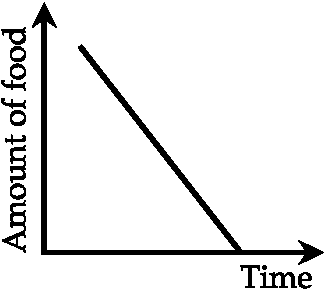
\includegraphics[height=2.5cm,width=2.5cm]{Net-June-20-12}
	\end{figure}
 Amount of food is decreasing at a constant rate hence it will become zero after a certain interval of time however long it may be. Finally there will be no food available and all the population will die.\\
		So the correct answer is \textbf{Option (a)}
\end{answer}
\item  A marksman had four successes in six attempts. What is the probability that he had three consecutive successes?
	 \begin{tasks}(4)
		\task[\textbf{a.}]$9 / 15$
		\task[\textbf{b.}] $12 / 15$
		\task[\textbf{c.}]$13 / 15$
		\task[\textbf{d.}] $6 / 15$
	\end{tasks}
\begin{answer}
	\begin{align*}
	\intertext{ Number of ways in which four successes can be obtained in 6 attempts ${ }^{6} C_{4}=15$. If there are four successes then there must be two failures. If the failures occurs on attempts 1 and 4 or 2 and 4 or 2 and 5 or 3 and 4 or 3 and 5 or 3 and 6 we can not get three consecutive successes. Hence there are $15-6=9$ ways of obtaining 3 consecutive successes.}
\text{	Required probability }&=\frac{9 / 64}{15 / 64}=\frac{9}{15}
	\end{align*}
		So the correct answer is \textbf{Option (a)}
\end{answer}
\item  The scores of the six students of Group A in an examination are 38, 45, 42, 58, 62 and 55 . In the same examination, the scores of the six students of Group B of size 7 are 38,41,44, 46, 49 and 52 , where one score is missing. If the arithmetic means of the scores of the two groups are same, then what is the missing score?
 \begin{tasks}(4)
	\task[\textbf{a.}]80
	\task[\textbf{b.}]65
	\task[\textbf{c.}]63
	\task[\textbf{d.}] 62
\end{tasks}
\begin{answer}
	\begin{align*}
	\text { The mean of group } \mathrm{A}&=\frac{38+45+42+58+62+55}{6}=50\\
\intertext{	From the question, the mean of group B is the same as the mean of group A. Therefore, if $x$ is the missing score then}
	\frac{38+41+44+46+49+52+x}{7}&=50 \quad \Rightarrow x=350-270=80
	\end{align*}
		So the correct answer is \textbf{Option (a)}
\end{answer}
\item  A wire is bent into the shape of a square enclosing an area $M$. If the same wire is bent to form a circle, the area enclosed will be
 \begin{tasks}(4)
	\task[\textbf{a.}]$\frac{4 \sqrt{2} M}{\pi}$
	\task[\textbf{b.}]$M$
	\task[\textbf{c.}] $\frac{4 M}{\pi}$
	\task[\textbf{d.}] $\frac{\pi M}{2 \sqrt{2}}$
\end{tasks}
\begin{answer}
	\begin{align*}
\text{The perimeter of square }&=4 \sqrt{M}\\
	\text{Now, circumference of circle }&=\text{ Perimeter of square}\\
	\Rightarrow 2 \pi r&=4 \sqrt{M} \Rightarrow r=\frac{2 \sqrt{M}}{\pi}\\
\text{	Area of circle }&=\pi r^{2}=\pi\left(\frac{2 \sqrt{M}}{\pi}\right)^{2}=\frac{4 M}{\pi}
	\end{align*}
		So the correct answer is \textbf{Option (c)}
\end{answer}
\item  In a flight of $600 \mathrm{~km}$, an aircraft was slowed down due to bad weather. Its average speed for the trip was reduced by $200 \mathrm{~km} / \mathrm{h}$ and the time of flight increased by 30 minutes. What was the scheduled duration of the flight?
 \begin{tasks}(4)
	\task[\textbf{a.}]1 hour
	\task[\textbf{b.}]1 hour 30 minutes
	\task[\textbf{c.}] 2 hours
	\task[\textbf{d.}] 45 minutes
\end{tasks}	
\begin{answer}
	\begin{align}
	\intertext{ Let the normal speed of aircraft be $v \mathrm{~km} / \mathrm{hr}$ and the scheduled duration of the flight be $t$ hours.}
\text{	From the question}\notag\\
	v t&=600\label{20-03}\\
\text{	and }(v-200)\left(t+\frac{1}{2}\right)&=600\label{20-04}\\
\text{	From equation (\ref{20-03}) and (\ref{20-04})}\notag\\
	v t+\frac{v}{2}-200 t-100&=v t \notag\\
	\Rightarrow \frac{v}{2}-200 t-100&=0\label{20-05}\\
\text{	Putting the value of $v$ }&\text{from equation (\ref{20-03}) into equation (\ref{20-05}) gives}\notag\\
	\frac{300}{t}-200 t-100&=0 \notag\\
	\Rightarrow 200 t^{2}+100 t-300&=0 \Rightarrow 2 t^{2}+t-3=0 \notag\\
	\Rightarrow 2 t^{2}-2 t+3 t-3&=0 \Rightarrow 2 t(t-1)+3(t-1)=0 \notag\\
	\Rightarrow(2 t+3)(t-1)&=0 \Rightarrow t=-\frac{3}{2} \text { or } t=1\notag\\
	\text{Since negative value of $t$ is}&\text{ unacceptable. Hence $t=1$ hour.}\notag
	\end{align}
		So the correct answer is \textbf{Option (a)}
\end{answer}
\section{PART B}	
\item  A point mass $m$, is constrained to move on the inner surface of a paraboloid of revolution $x^{2}+y^{2}=a z$ (where $a>0$ is a constant). When it spirals down the surface, under the influence of gravity (along $-z$ direction), the angular speed about the $z$ - axis is proportional to
 \begin{tasks}(2)
	\task[\textbf{a.}]1 (independent of $z$ )
	\task[\textbf{b.}] $z$
	\task[\textbf{c.}]$z^{-1}$
	\task[\textbf{d.}] $z^{-2}$
\end{tasks}
\begin{answer}
	\begin{align*}
	\text { Using Lagrangian}&\text{ in cylindrical coordinate }\\
	L&=\frac{1}{2} m\left(\dot{r}^{2}+r^{2} \dot{\theta}^{2}+\dot{z}^{2}\right)-m g z \quad\\\text{ with constraint } x^{2}+y^{2}&=a z \Rightarrow r^{2}=a z \Rightarrow \dot{z}=\frac{2 r \dot{r}}{a}\\
	 L&=\frac{1}{2} m\left(\dot{r}^{2}+r^{2} \dot{\theta}^{2}+\left(\frac{2 r \dot{r}}{a}\right)^{2}\right)-\frac{m g r^{2}}{a}\\
	\text{$\theta$ is cyclic coordinate so }\frac{\partial L}{\partial \theta}&=0 \Rightarrow \frac{\partial L}{\partial \dot{\theta}}=J \Rightarrow m r^{2} \dot{\theta}=J \Rightarrow \dot{\theta} \propto \frac{1}{r^{2}} \propto \frac{1}{z}
	\end{align*}
	So the correct answer is \textbf{Option (c)}
\end{answer}
\item  Two coupled oscillators in a potential $V(x, y)=\frac{1}{2} k x^{2}+2 x y+\frac{1}{2} k y^{2}(k>2)$ can be decoupled into two independent harmonic oscillators (coordinates: $x^{\prime}, y^{\prime}$ ) by means of an appropriate transformation $\left(\begin{array}{l}x^{\prime} \\ y^{\prime}\end{array}\right)=S\left(\begin{array}{l}x \\ y\end{array}\right)$. The transformation matrix $S$ is
 \begin{tasks}(2)
	\task[\textbf{a.}]$\left(\begin{array}{cc}\frac{1}{\sqrt{2}} & 1 \\ 1 & -\frac{1}{\sqrt{2}}\end{array}\right)$
	\task[\textbf{b.}]$\left(\begin{array}{cc}\frac{1}{\sqrt{2}} & -\frac{1}{\sqrt{2}} \\ \frac{1}{\sqrt{2}} & \frac{1}{\sqrt{2}}\end{array}\right)$
	\task[\textbf{c.}]$\left(\begin{array}{cc}\frac{1}{\sqrt{2}} & -\frac{1}{\sqrt{2}} \\ -\frac{1}{\sqrt{2}} & \frac{1}{\sqrt{2}}\end{array}\right)$
	\task[\textbf{d.}] $\left(\begin{array}{cc}0 & -1 \\ 1 & 0\end{array}\right)$
\end{tasks}
\begin{answer}
	\begin{align*}
\intertext{ The normal mode of given potential is $\left(\begin{array}{c}\frac{1}{\sqrt{2}} \\ \frac{1}{\sqrt{2}}\end{array}\right)$ and $\left(\begin{array}{c}-\frac{1}{\sqrt{2}} \\ \frac{1}{\sqrt{2}}\end{array}\right)$ in the basis of normal mode the potential can be diagonalise.}
	\end{align*}
	So the correct answer is \textbf{Option (b)}
\end{answer}
\item  A heavy particle of rest mass $M$ while moving along the positive $z$-direction, decays into two identical light particles with rest mass $m$ (where $M>2 m$ ). The maximum value of the momentum that any one of the lighter particles can have in a direction perpendicular to the $z$ direction, is
 \begin{tasks}(2)
	\task[\textbf{a.}] $\frac{1}{2} C \sqrt{M^{2}-4 m^{2}}$
	\task[\textbf{b.}]$\frac{1}{2} C \sqrt{M^{2}-2 m^{2}}$
	\task[\textbf{c.}] $C \sqrt{M^{2}-4 m^{2}}$
	\task[\textbf{d.}]$\frac{1}{2} M C$ 
\end{tasks}
\begin{answer}$\left. \right. $
		\begin{figure}[H]
		\centering
		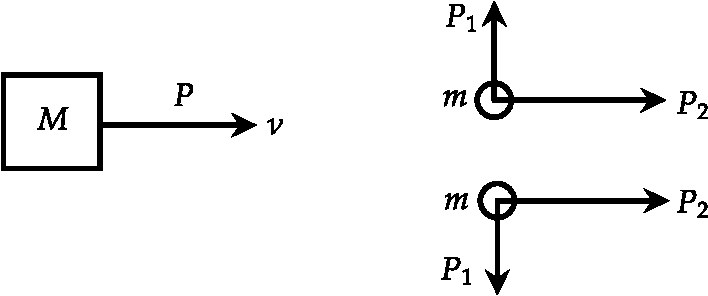
\includegraphics[height=2.5cm,width=6cm]{Net-June-20-13}
	\end{figure}
	Let $P$ be the momentum of heavy mass $M$. And let $P_{1}$ be the momentum of the light particles of mass $m$ in the direction perpendicular to $z$ and $P_{2}$ be the momentum in $z$-direction.\\
	According to conservation of momentum,
	\begin{align*}
	\text{Momentum of mass }M, P&=P_{2}+P_{2}=2 P_{2} \Rightarrow P_{2}=P / 2\\
\text{	Energy of mass } M, \quad E&=\sqrt{P^{2} c^{2}+M^{2} c^{4}}\\
\text{	Momentum of a mass } m,&=\sqrt{P_{1}^{2}+P_{2}^{2}}=\sqrt{P_{1}^{2}+\frac{P^{2}}{4}}\\
\text{	Energy of mass }m, E_{1}^{2}&=\left(P_{1}^{2}+\frac{P^{2}}{4}\right) c^{2}+m^{2} c^{4}\\
	\text{As energy is conserved }E&=E_{1}+E_{2}=2 E_{1} \Rightarrow E_{1}=\frac{E}{2}\qquad \because E_{1}=E_{2}\\
\text{	Thus } E_{1}^{2}&=\frac{E^{2}}{4}=\left(P_{1}^{2}+\frac{P^{2}}{4}\right) c^{2}+m^{2} c^{4} \quad \Rightarrow 4\left(P_{1}^{2}+\frac{P^{2}}{4}\right) c^{2}+4 m^{2} c^{4}=P^{2} c^{2}+M^{2} c^{4} \\
4 P_{1}^{2} c^{2}+P^{2} c^{2}+4 m^{2} c^{4}&=P^{2} c^{2}+M^{2} c^{4} \Rightarrow 4 P_{1}^{2} c^{2}+4 m^{2} c^{4}=M^{2} c^{4} \Rightarrow 4 P_{1}^{2}=M^{2} c^{2}-4 m^{2} c^{2}\\ P_{1}^{2}&=\frac{c^{2}}{4}\left(M^{2}-4 m^{2}\right) \Rightarrow P_{1}=\frac{c}{2} \sqrt{M^{2}-4 m^{2}}
	\end{align*}
		So the correct answer is \textbf{Option (a)}
\end{answer}
\item A frictionless horizontal circular table is spinning with a uniform angular velocity $\omega$ about the vertical axis through its centre. If a ball of radius $a$ is placed on it at a distance $r$ from the centre of the table, its linear velocity will be
 \begin{tasks}(2)
	\task[\textbf{a.}]$-r \omega \hat{r}+a \omega \hat{\theta}$
	\task[\textbf{b.}]$r \omega \hat{r}+a \omega \hat{\theta}$
	\task[\textbf{c.}]$a \omega \hat{r}+r \omega \hat{\theta}$
	\task[\textbf{d.}]  0 (zero)
\end{tasks}
\begin{answer}
 Since table is frictionless then there is not any tangential force, so ball will have zero speed. \\
	So the correct answer is \textbf{Option (d)}
\end{answer}
\item An inductor $L$, a capacitor $C$ and a resistor $R$ are connected in series to an $A C$ source, $V=V_{0} \sin \omega t$. If the net current is found to depend only on $R$, then
 \begin{tasks}(2)
	\task[\textbf{a.}]$C=0$
	\task[\textbf{b.}]$L=0$
	\task[\textbf{c.}]$\omega=1 / \sqrt{L C}$
	\task[\textbf{d.}]$\omega=\sqrt{\frac{1}{L C}-\frac{R^{2}}{4 L^{2}}}$ 
\end{tasks}
\begin{answer}
	\begin{align*}
	\text{The net current}&\text{ is found to depend only on $R$,}\\
	\text { if } X_{L}&=X_{C} \Rightarrow \omega L=\frac{1}{\omega C} \Rightarrow \omega=\frac{1}{\sqrt{L C}}
	\end{align*}
		So the correct answer is \textbf{Option (c)}
\end{answer}
\item Three point charges $q$ are placed at the corners of an equilateral triangle. Another point charge $-Q$ is placed at the centroid of the triangle. If the force on each of the charges $q$ vanishes, then the ratio $Q / q$ is
 \begin{tasks}(4)
	\task[\textbf{a.}]$\sqrt{3}$
	\task[\textbf{b.}]$\frac{1}{\sqrt{3}}$
	\task[\textbf{c.}]$\frac{1}{3 \sqrt{3}}$
	\task[\textbf{d.}]$\frac{1}{3}$ 
\end{tasks}
\begin{answer}$\left. \right. $
		\begin{figure}[H]
		\centering
		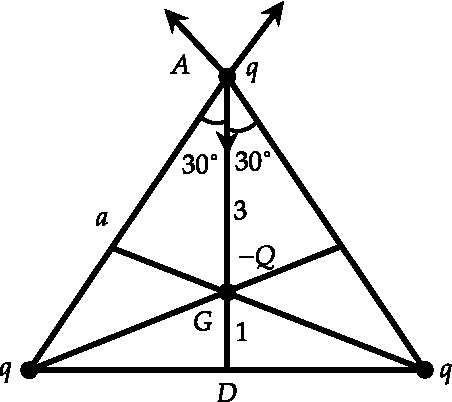
\includegraphics[height=4cm,width=4.2cm]{Net-June-20-14}
	\end{figure}
	\begin{align*}
 D G&=\frac{1}{3} A D=\frac{1}{3} \times \frac{\sqrt{3}}{2} a\\
	A G&=A D-D G=\frac{2}{3} A D=\frac{2}{3} \times \frac{\sqrt{3}}{2} a \Rightarrow A G=\frac{a}{\sqrt{3}}\\
	&\text{Force on charge $q$ is zero so}\\
	\frac{k q^{2}}{a^{2}} \cos 30^{\circ}+\frac{k q^{2}}{a^{2}} \cos 30^{\circ}&=k \frac{q Q}{(a / \sqrt{3})^{2}} \\
	q \frac{\sqrt{3}}{2}+\frac{q \sqrt{3}}{2}&=3 Q \Rightarrow \frac{Q}{q}=\frac{\sqrt{3}}{3}=\frac{1}{\sqrt{3}}
	\end{align*}
		So the correct answer is \textbf{Option (b)}
\end{answer}
\item Three infinitely long wires, each carrying equal current are placed in the $x y$-plane along $x=0,+d$ and $-d$. On the $x y$ - plane, the magnetic field vanishes at
 \begin{tasks}(2)
	\task[\textbf{a.}]$x=\pm \frac{d}{2}$
	\task[\textbf{b.}]$x=\pm d\left(1+\frac{1}{\sqrt{3}}\right)$
	\task[\textbf{c.}] $x=\pm d\left(1-\frac{1}{\sqrt{3}}\right)$
	\task[\textbf{d.}] $x=\pm \frac{d}{\sqrt{3}}$
\end{tasks}	
\begin{answer}$\left. \right. $
		\begin{figure}[H]
		\centering
		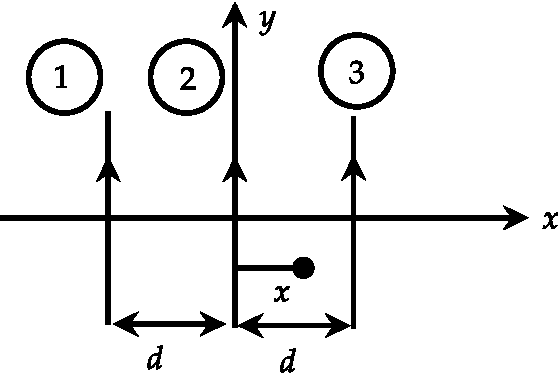
\includegraphics[height=3cm,width=4.5cm]{Net-June-20-15}
	\end{figure}
	\begin{align*}
	&B_{1}+B_{2}=B_{3}\\
	&\frac{\mu_{0} I}{2 \pi(d+x)}+\frac{\mu_{0} I}{2 \pi x}=\frac{\mu_{0} I}{2 \pi(d-x)} \\
	&\Rightarrow \frac{1}{d+x}+\frac{1}{x}=\frac{1}{d-x} \Rightarrow \frac{x+d+x}{x(d+x)}=\frac{1}{(d-x)} \\
	&\Rightarrow(d+2 x)(d-x)=d x+x^{2} \\
	&\Rightarrow d^{2}-x d+2 x d-2 x^{2}=d x+x^{2} \\
	&\Rightarrow d^{2}+x d-2 x^{2}=d x+x^{2} \\
	&\Rightarrow 3 x^{2}=d^{2} \Rightarrow x=\pm \frac{d}{\sqrt{3}}
	\end{align*}
	So the correct answer is \textbf{Option (d)}
\end{answer}
\item The following figure shows the intensity of the interference pattern in the Young's double-slit experiment with two slits of equal width is observed on a distant screen	
	\begin{figure}[H]
	\centering
	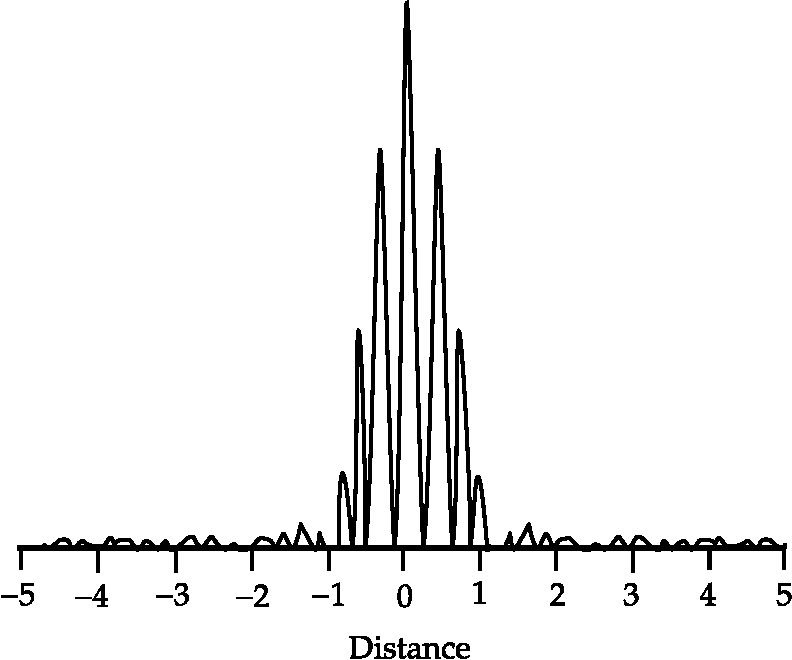
\includegraphics[height=5cm,width=5.5cm]{Net-June-20-16}
\end{figure}
If the separation between the slits is doubled and the width of each of the slits is halved, then the new interference pattern is best represented by 
\begin{tasks}(2)
	\task[\textbf{a.}]
		\begin{figure}[H]
		\centering
		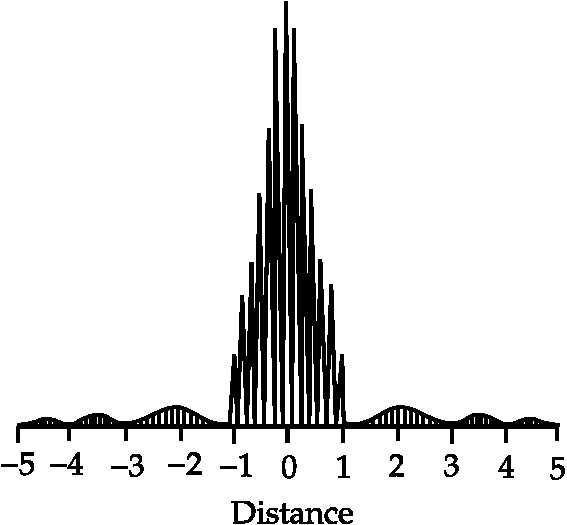
\includegraphics[height=5cm,width=5.5cm]{Net-June-20-17}
	\end{figure}
	\task[\textbf{b.}]
		\begin{figure}[H]
		\centering
		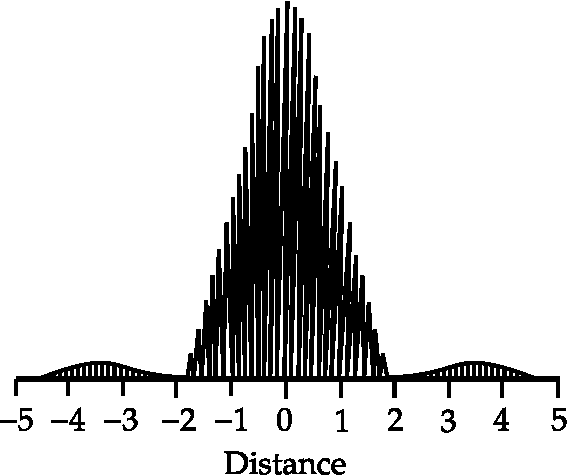
\includegraphics[height=5cm,width=5.5cm]{Net-June-20-18}
	\end{figure}
	\task[\textbf{c.}]
		\begin{figure}[H]
		\centering
		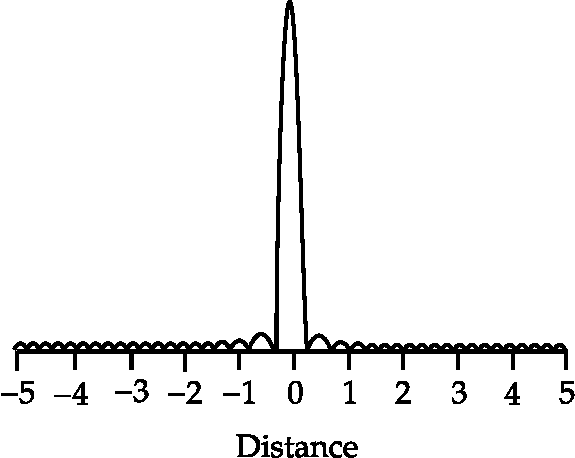
\includegraphics[height=5cm,width=5.5cm]{Net-June-20-19}
	\end{figure}
	\task[\textbf{d.}] 
		\begin{figure}[H]
		\centering
		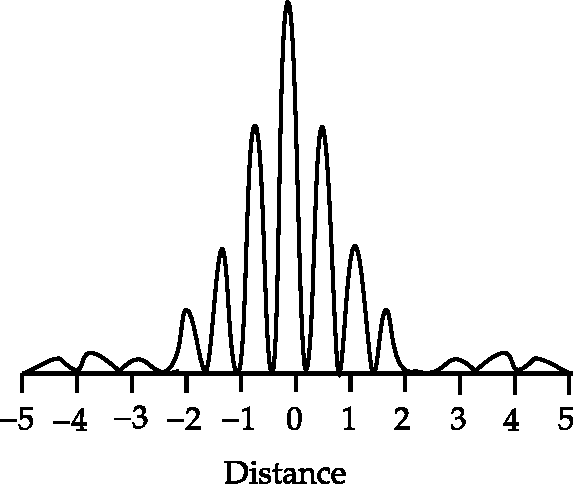
\includegraphics[height=5cm,width=5.5cm]{Net-June-20-20}
	\end{figure}
\end{tasks}
\begin{answer}
	\begin{align*}
	\text { (i) } \beta&=\frac{D \lambda}{d}\\
&\text{	As $d$ is increased to $2 d$, so $\beta$ will be halved.}\\
	&\text{(ii) As slit width $e$ is reduced to $e / 2$ so width of central envelop will be increased.}
	\end{align*}
		So the correct answer is \textbf{Option (b)}
\end{answer}
\item  Let $\vec{E}(x, y, z, t)=\vec{E}_{0} \cos (2 x+3 y-\omega t)$, where $\omega$ is a constant, be the electric field of an electromagnetic wave travelling in vacuum. Which of the following vectors is a valid choice for $\vec{E}_{0} ?$	
 \begin{tasks}(4)
	\task[\textbf{a.}] $\hat{i}-\frac{3}{2} \hat{j}$
	\task[\textbf{b.}]$\hat{i}+\frac{3}{2} \hat{j}$
	\task[\textbf{c.}]$\hat{i}+\frac{2}{3} \hat{j}$
	\task[\textbf{d.}] $\hat{i}-\frac{2}{3} \hat{j}$
\end{tasks}
\begin{answer}
	\begin{align*}
\vec{K}&=2 \hat{x}+3 \hat{y}\\
	\therefore\quad \vec{K} \cdot \vec{E}&=0 \Rightarrow \vec{E}_{0} \rightarrow \hat{x}-\frac{2}{3} \hat{y}
	\end{align*}
		So the correct answer is \textbf{Option (d)}
\end{answer}
\item Two time dependent non-zero vectors $\vec{u}(t)$ and $\vec{v}(t)$, which are not initially parallel to each other, satisfy $\vec{u} \times \frac{d \vec{v}}{d t}-\vec{v} \times \frac{d \vec{u}}{d t}=0$ at all time $t$. If the area of the parallelogram formed by $\vec{u}(t)$ and $\vec{v}(t)$ be $A(t)$ and the unit normal vector to it be $\hat{n}(t)$, then
 \begin{tasks}(1)
	\task[\textbf{a.}] A(t) increases linearly with $t$, but $\hat{n}(t)$ is a constant
	\task[\textbf{b.}] $A(t)$ increases linearly with $t$, and $\hat{n}(t)$ rotates about $\vec{u}(t) \times \vec{v}(t)$
	\task[\textbf{c.}]$A(t)$ is a constant, but $\hat{n}(t)$ rotates about $\vec{u}(t) \times \vec{v}(t)$
	\task[\textbf{d.}] $A(t)$ and $\hat{n}(t)$ are constants
\end{tasks}
\begin{answer}
	\begin{align*}
	 \vec{A}(t)&=\vec{u} \times \vec{v}, \quad \hat{n}(t)=\frac{\vec{u} \times \vec{v}}{|\vec{u} \times \vec{v}|}=\frac{1}{A} \vec{u} \times \vec{v}\\
	\Rightarrow \frac{d \hat{n}}{d t}&=\frac{1}{A} \vec{u} \times \frac{d \vec{v}}{d t}+\frac{1}{A} \frac{d \vec{u}}{d t} \times \vec{v}=\frac{1}{A}\left(\vec{u} \times \frac{d \vec{v}}{d t}-\vec{v} \times \frac{d \vec{u}}{d t}\right)=0 \\
	\Rightarrow \hat{n}(t)&=\text { const } \\
	\Rightarrow A(t)&=|\vec{u} \times \vec{v}|=\text { const }
	\end{align*}
		So the correct answer is \textbf{Option (d)}
\end{answer}
\item A basket consists of an infinite number of red and black balls in the proportion $p:(1-p)$. Three balls are drawn at random without replacement. The probability of their being two red and one black is a maximum for
 \begin{tasks}(4)
	\task[\textbf{a.}]$p=\frac{3}{4}$
	\task[\textbf{b.}]$p=\frac{3}{5}$
	\task[\textbf{c.}] $p=\frac{1}{2}$
	\task[\textbf{d.}] $p=\frac{2}{3}$ 
\end{tasks}
\begin{answer}
	\begin{align*}
	P=p^{2}(1-p) \quad \Rightarrow \frac{d P}{d p}&=\frac{d}{d p} p^{2}(1-p)=0 \Rightarrow p^{2}(-1)+(1-p) 2 p=0\\
	\Rightarrow-p^{2}+2 p-2 p^{2}&=0 \Rightarrow 3 p^{2}=2 p \quad \Rightarrow p=2 / 3
	\end{align*}
	So the correct answer is \textbf{Option (d)}
\end{answer}
\item The eigenvalues of the $3 \times 3$ matrix $M=\left(\begin{array}{lll}a^{2} & a b & a c \\ a b & b^{2} & b c \\ a c & b c & c^{2}\end{array}\right)$ are
 \begin{tasks}(2)
	\task[\textbf{a.}]$a^{2}+b^{2}+c^{2}, 0,0$
	\task[\textbf{b.}]$b^{2}+c^{2}, a^{2}, 0$
	\task[\textbf{c.}]$a^{2}+b^{2}, c^{2}, 0$
	\task[\textbf{d.}]$a^{2}+c^{2}, b^{2}, 0$	 
\end{tasks}
\begin{answer}
	\begin{align*}
	M&=\left(\begin{array}{lll}
	a^{2} & a b & a c \\
	a b & b^{2} & b c \\
	a c & b c & c^{2}
	\end{array}\right)\\
\text{	To make it simple, Let }a&=1, b=1, c=1\text{ so }
	M=\left[\begin{array}{lll}
	1 & 1 & 1 \\
	1 & 1 & 1 \\
	1 & 1 & 1
	\end{array}\right]_{3 \times 3}\\
	\Rightarrow \lambda&=3,0,0
	\end{align*}
		So the correct answer is \textbf{Option (a)}
\end{answer}
\item  A function of a complex variable $z$ is defined by the integral $f(z)=\oint_{\Gamma} \frac{w^{2}-2}{w-z} d w$, where $\Gamma$ is a circular contour of radius 3 , centred at origin, running counter-clockwise in the $w$-plane. The value of the function at $z=(2-i)$ is
 \begin{tasks}(4)
	\task[\textbf{a.}]0
	\task[\textbf{b.}]$1-4 i$
	\task[\textbf{c.}]$8 \pi+2 \pi i$
	\task[\textbf{d.}]$-\frac{2}{\pi}-\frac{i}{2 \pi}$ 
\end{tasks}	
\begin{answer}$\left. \right. $
		\begin{figure}[H]
		\centering
		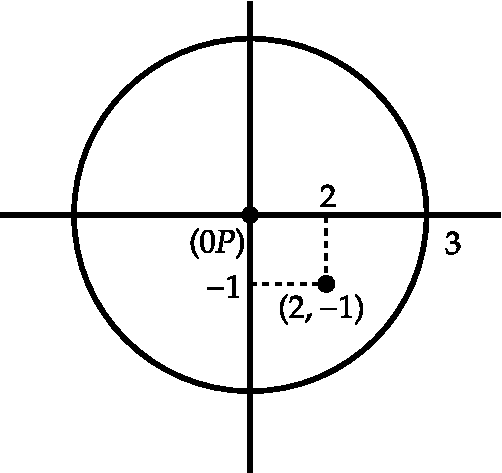
\includegraphics[height=4cm,width=4.4cm]{Net-June-20-21}
	\end{figure}
	\begin{align*}
	 f(z)&=\oint_{\Gamma} \frac{w^{2}-2}{w-z} d w \\
	 \omega&=z is \text{a simple pole.}\\
	\text{Residue }\lim _{\omega \rightarrow z}(\omega-z) \frac{\left(\omega^{2}-2\right)}{(\omega-z)}&=(2-i)^{2}-2=4-1-4 i-2=(1-4 i)\\
	f(z)&=\oint_{\Gamma} \frac{w^{2}-2}{w-z} d w=2 \pi i(1-4 i)=2 \pi i+8 \pi
	\end{align*}
	So the correct answer is \textbf{Option (c)}
\end{answer}
\item  The temperatures of two perfect black bodies $A$ and $B$ are $400 K$ and $200 K$, respectively. If the surface area of $A$ is twice that of $B$, the ratio of total power emitted by $A$ to that by $B$ is
 \begin{tasks}(4)
	\task[\textbf{a.}]4
	\task[\textbf{b.}]2
	\task[\textbf{c.}]32
	\task[\textbf{d.}] 16
\end{tasks}
\begin{answer}
	\begin{align*}
	A \rightarrow 400 K, &\quad B \rightarrow 200 K\\
	\text { Energy densities, } \frac{u_{A}}{u_{B}}&=\frac{400^{4}}{200^{4}}=\frac{4^{4}}{2^{4}}=\frac{4 \times 4 \times 4 \times 4}{2 \times 2 \times 2 \times 2}=16, \frac{P_{A}}{P_{B}}=\frac{u_{A} 2 A}{u_{B} A}=2 * 16=32
	\end{align*}
	So the correct answer is \textbf{Option (c)}
\end{answer}
\item Two ideal gases in a box are initially separated by a partition. Let $N_{1}, V_{1}$ and $N_{2}, V_{2}$ be the numbers of particles and volume occupied by the two systems. When the partition is removed, the pressure of the mixture at an equilibrium temperature $T$, is
 \begin{tasks}(2)
	\task[\textbf{a.}]$k_{B} T\left(\frac{N_{1}+N_{2}}{2\left(V_{1}+V_{2}\right)}\right)$
	\task[\textbf{b.}]$k_{B} T\left(\frac{N_{1}+N_{2}}{V_{1}+V_{2}}\right)$
	\task[\textbf{c.}]$k_{B} T\left(\frac{N_{1}}{V_{1}}+\frac{N_{2}}{V_{2}}\right)$
	\task[\textbf{d.}] $\frac{1}{2} k_{B} T\left(\frac{N_{1}}{V_{1}}+\frac{N_{2}}{V_{2}}\right)$
\end{tasks}
\begin{answer}
	\begin{align*}
	\renewcommand*{\arraystretch}{1.5}
	\begin{array}{|c|c|}
	\hline N_{1}, V_{1} & N_{2}, V_{2} \\
	P_{1} & P_{2} \\
	\hline
	\end{array}\\
\text{	Finally, At equilibrium }P\left(V_{1}+V_{2}\right)&=n R T, n\text{ is number of moles }=\frac{N}{N_{A}}\\
	P=\frac{n R T}{V_{1}+V_{2}} ; \quad n&=n_{1}+n_{2} ; \quad n=\frac{N_{1}}{N_{A}}+\frac{N_{2}}{N_{A}}, k_{B}=\frac{R}{N_{A}} \\
	P=\frac{\left(N_{1}+N_{2}\right) k_{B} T}{V_{1}+V_{2}}&=k_{B} T\left(\frac{N_{1}+N_{2}}{V_{1}+V_{2}}\right)
	\end{align*}
		So the correct answer is \textbf{Option (b)}
\end{answer}
\item An idealised atom has a non-degenerate ground state at zero energy and a $g$-fold degenerate excited state of energy $E$. In a non-interacting system of $N$ such atoms, the population of the excited state may exceed that of the ground state above a temperature $T>\frac{E}{2 k_{B} \ln 2}$. The minimum value of $g$ for which this is possible is
 \begin{tasks}(4)
	\task[\textbf{a.}]8
	\task[\textbf{b.}]4
	\task[\textbf{c.}]2
	\task[\textbf{d.}] 1
\end{tasks}
\begin{answer}$\left. \right. $
		\begin{figure}[H]
		\centering
		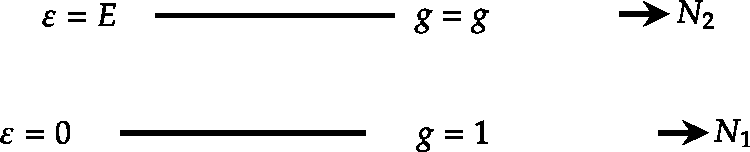
\includegraphics[height=1.3cm,width=6cm]{Net-June-20-22}
	\end{figure}
	\begin{align*}
	z&=1+g e^{-\beta \varepsilon} \\
	P_{1}&=\frac{e^{-\beta 0}}{z}, \quad P_{2}=\frac{g e^{-\beta \varepsilon}}{z} \\
	N_{1}&=P_{1} N, N_{2}=P_{2} N \\
	N_{2}&=N_{1} \Rightarrow g \frac{e^{-\beta \varepsilon}}{z}=\frac{1}{z} \Rightarrow g \cdot \bar{e}^{E / k_{B} T}=1 \Rightarrow g \cdot \bar{e}^{E / k_{B}\left(E /\left(2 k_{B} \ln 2\right)\right.}=1 \\
	\Rightarrow g&=e^{\ln 2^{2}}=4
	\end{align*}
		So the correct answer is \textbf{Option (b)}
\end{answer}
\item  The Hamiltonian of a system of $N$ non-interacting particles, each of mass $m$, in one dimension is
$$
H=\sum_{i=1}^{N}\left(\frac{p_{i}^{2}}{2 m}+\frac{\lambda}{4} x_{i}^{4}\right)
$$
where $\lambda>0$ is a constant and $p_{i}$ and $x_{i}$ are the momentum and position respectively of the $i$-th particle. The average internal energy of the system is
 \begin{tasks}(4)
	\task[\textbf{a.}]$\frac{4}{3} k_{B} T$
	\task[\textbf{b.}]$\frac{3}{4} k_{B} T$
	\task[\textbf{c.}] $\frac{3}{2} k_{B} T$
	\task[\textbf{d.}] $\frac{1}{3} k_{B} T$
\end{tasks}	
\begin{answer}
	\begin{align*}
	H&=\sum_{i=1}^{N}\left(\frac{p_{i}^{2}}{2 m}+\frac{\lambda}{4} x_{i}^{4}\right), \quad\left\langle\frac{p_{i}^{2}}{2 m}\right\rangle=\frac{1}{2} k_{B} T, \quad\left\langle\frac{\lambda}{4} x_{i}^{4}\right\rangle=\frac{\int_{-\infty}^{\infty} e^{-\beta \frac{\lambda}{4} x^{4}} \frac{\lambda}{4} x^{4} d x}{\int_{-\infty}^{\infty} e^{-\beta \frac{\lambda}{4} x^{4}} d x}\\
	\int_{0}^{\infty} e^{-b x^{4}} d x&=\frac{\sqrt{5 / 4}}{b^{1 / 4}}, \quad b \geq 0 \quad \text { and } \quad \int_{0}^{\infty} b x^{4} e^{-b x^{4}} d x=\frac{\sqrt{5 / 4}}{4 b^{1 / 4}}\\
	\langle E\rangle&=\frac{1}{2} k_{B} T+\frac{1}{4} k_{B} T=\frac{2+1}{4} k_{B} T=\frac{3}{4} k_{B} T
	\end{align*}
	So the correct answer is \textbf{Option (b)}
\end{answer}
\item A $10 \mathrm{~V}$ battery is connected in series to a resistor $R$ and a capacitor $C$, as shown the figure.
\begin{figure}[H]
	\centering
	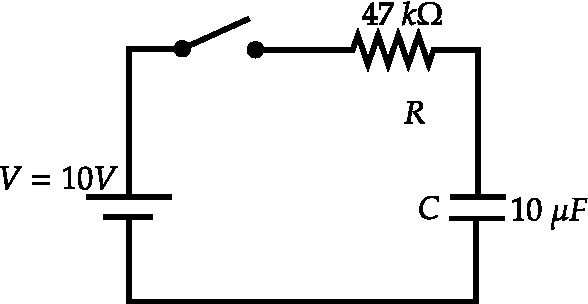
\includegraphics[height=2.5cm,width=5cm]{Net-June-20-23}
\end{figure}
The initial charge on the capacitor is zero. The switch is turned on and the capacitor is allowed to charge to its full capacity. The total work done by the battery in this process is
 \begin{tasks}(4)
	\task[\textbf{a.}]$10^{-3} \mathrm{~J}$
	\task[\textbf{b.}]$2 \times 10^{-3} \mathrm{~J}$
	\task[\textbf{c.}]$5 \times 10^{-4} \mathrm{~J}$
	\task[\textbf{d.}] $47 \times 10^{-2} J$
\end{tasks}
\begin{answer}
	\begin{align*}
&\text{ The total work done by the battery in this process is}\\
	W&=q V=(C V) V=C V^{2}=10 \times 10^{-6} \times(10)^{2}=10^{-3} \text { Joules }
	\end{align*}
		So the correct answer is \textbf{Option (A)}
\end{answer}
\item In the 3-bit register shown below, $Q_{1}$ and $Q_{3}$ are the least and the most significant bits of the output, respectively.
\begin{figure}[H]
	\centering
	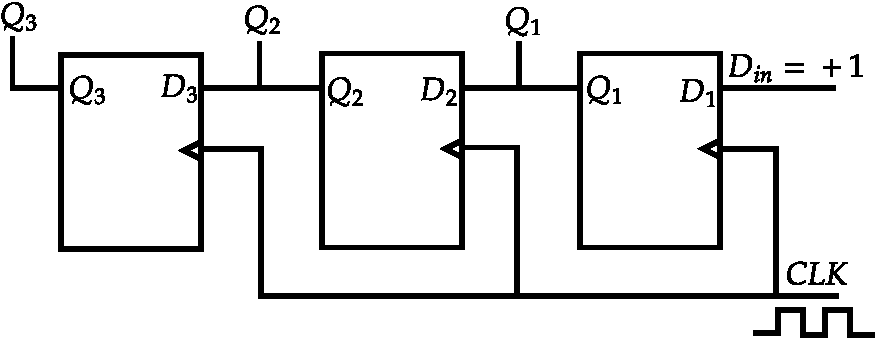
\includegraphics[height=3cm,width=7cm]{Net-June-20-24}
\end{figure}
If $Q_{1}, Q_{2}$ and $Q_{3}$ are set to zero initially, then the output after the arrival of the second falling clock (CLK) edge is
 \begin{tasks}(4)
	\task[\textbf{a.}]001
	\task[\textbf{b.}]100
	\task[\textbf{c.}]011
	\task[\textbf{d.}] 110 
\end{tasks}
\begin{answer}
	\begin{align*}
	\begin{array}{|ccc|c}
	\cline{1-3} Q_{3} & Q_{3} & Q_{1}& \\
	\cline{1-3} 0 & 0 & 1 &(1)\\
	\cline{1-3} 0 & 1 & 1 &(2)\\
	\cline{1-3}
	\end{array}
	\end{align*}
	So the correct answer is \textbf{Option (c)}
\end{answer}
\item The Boolean equation $Y=\bar{A} B C+\bar{A} B \bar{C}+A \bar{B} \bar{C}+A \bar{B} C$ is to be implemented using only twoinput NAND gates. The minimum number of gates required is
 \begin{tasks}(4)
	\task[\textbf{a.}]3
	\task[\textbf{b.}]4
	\task[\textbf{c.}]5
	\task[\textbf{d.}] 6
\end{tasks}
\begin{answer}
	\begin{align*}
	Y&=\bar{A} B C+\bar{A} B \bar{C}+A \bar{B} \bar{C}+A \bar{B} C \quad \Rightarrow Y=\bar{A} B(C+\bar{C})+A \bar{B}(\bar{C}+C)\\
	\Rightarrow Y&=\bar{A} B+A \bar{B}\\
	\text { Implementing}&\text{ Ex-OR Gate }
	\end{align*}
	\begin{figure}[H]
		\centering
		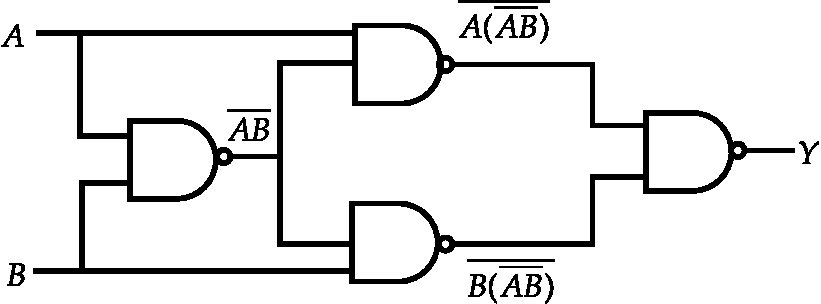
\includegraphics[height=3cm,width=7.5cm]{Net-June-20-26}
	\end{figure}
	\begin{align*}
	\Rightarrow Y&=\overline{(A(\overline{A B}))(B(\overline{A B}))}=\overline{A(\overline{A B})}+\overline{B(\overline{A B})} Y=A(\bar{A}+\bar{B})+B(\bar{A}+\bar{B}) \\
	Y&=A \bar{B}+\bar{A} B\\
	\text { So minimum } 4& \text { number of gates are required. }
	\end{align*}
		So the correct answer is \textbf{Option (b)}
\end{answer}
\item  The temperature variation of the resistivity of four materials are shown in the following graphs.
 \begin{tasks}(2)
	\task[\textbf{a.}]
	\begin{figure}[H]
		\centering
		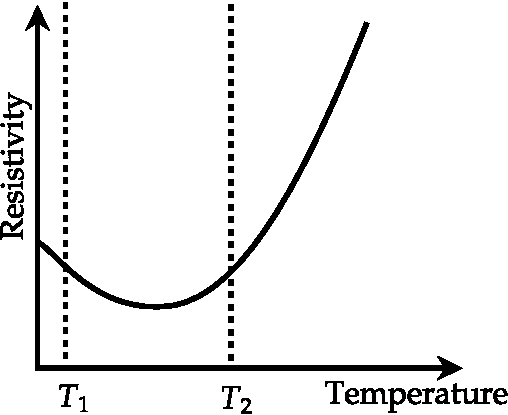
\includegraphics[height=3.5cm,width=4cm]{Net-June-20-27}
	\end{figure}
	\task[\textbf{b.}]
		\begin{figure}[H]
		\centering
		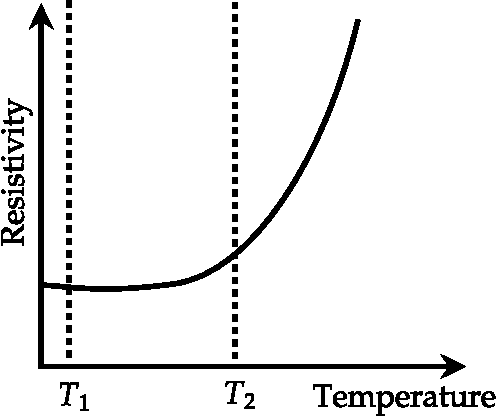
\includegraphics[height=3.5cm,width=4cm]{Net-June-20-28}
	\end{figure}
	\task[\textbf{c.}]
		\begin{figure}[H]
		\centering
		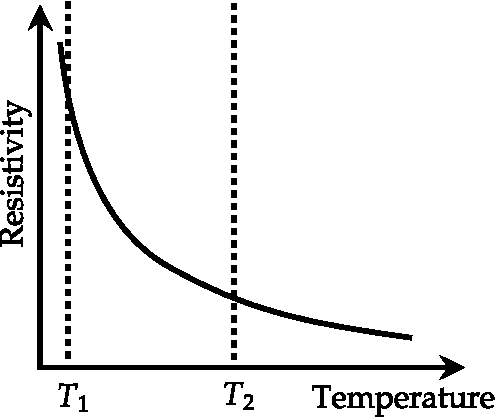
\includegraphics[height=3.5cm,width=4cm]{Net-June-20-29}
	\end{figure}
	\task[\textbf{d.}] 
		\begin{figure}[H]
		\centering
		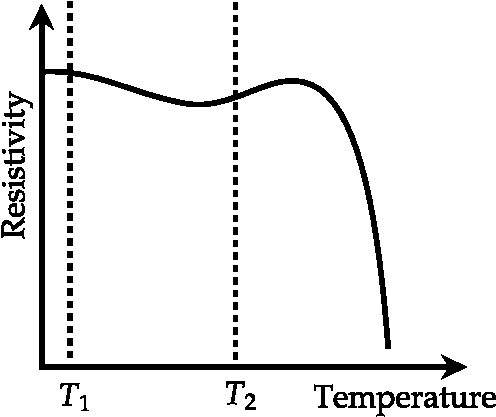
\includegraphics[height=3.5cm,width=4cm]{Net-June-20-30}
	\end{figure}
\end{tasks}	
The material that would make the most sensitive temperature sensor, when used at temperatures between $T_{1}$ and $T_{2}$, is
 \begin{tasks}(4)
	\task[\textbf{a.}]$\mathrm{A}$
	\task[\textbf{b.}]$\mathrm{B}$
	\task[\textbf{c.}]$\mathrm{C}$
	\task[\textbf{d.}] D
\end{tasks}	
\begin{answer}
 For the temperature sensor, the variation in the resistivity of material should be as large as possible without any local maximum or minimum. Option (a) \& (d) shows minimum while in (b) gradient is very low in comparison to $(\mathrm{C})$. Thus option (c) is the correct answer\\
		So the correct answer is \textbf{Option (c)}
\end{answer}
\item  Let $|n\rangle$ denote the energy eigenstates of a particle in a one-dimensional simple harmonic potential $V(x)=\frac{1}{2} m \omega^{2} x^{2}$\\
If the particle is initially prepared in the state $|\psi(t=0)\rangle=\sqrt{\frac{1}{2}}(|0\rangle+|1\rangle)$, the minimum time after which the oscillator will be found in the same state is
 \begin{tasks}(4)
	\task[\textbf{a.}]$3 \pi /(2 \omega)$
	\task[\textbf{b.}]$\pi / \omega$
	\task[\textbf{c.}]$\pi /(2 \omega)$
	\task[\textbf{d.}] $2 \pi / \omega$
\end{tasks}
\begin{answer}
	\begin{align*}
	|\psi(t=0)\rangle&=\sqrt{\frac{1}{2}}(|0\rangle+|1\rangle), \qquad|\psi(t=t)\rangle=\sqrt{\frac{1}{2}}\left(|0\rangle e^{-\frac{i \omega t}{2}}+|1\rangle e^{\frac{i 3 \omega t}{2}}\right)\\
	|\langle\psi(t) \mid \psi(0)\rangle|^{2}&=1 \Rightarrow\left|\frac{1}{2}\left(\exp -\frac{i \omega t}{2}+\exp -\frac{3 i \omega t}{2}\right)\right|^{2}=1 \\
	|1+\exp (-i \omega t)|^{2}&=4 \Rightarrow t=\frac{2 \pi}{\omega}
	\end{align*}
		So the correct answer is \textbf{Option (d)}
\end{answer}
\item  For the one dimensional potential wells $A, B$ and $C$, as shown in the figure, let $E_{A}, E_{B}$ and $E_{C}$ denote the ground sate energies of a particle, respectively.
	\begin{figure}[H]
	\centering
	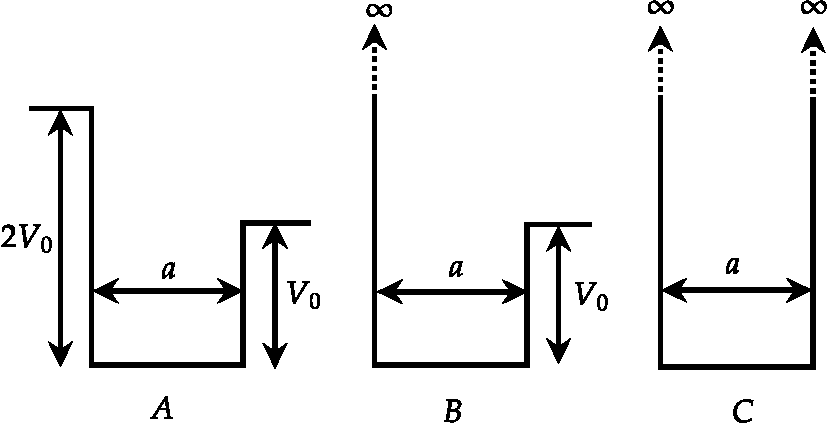
\includegraphics[height=3.2cm,width=6cm]{Net-June-20-31}
\end{figure}	
The correct ordering of the energies is
 \begin{tasks}(2)
	\task[\textbf{a.}] $E_{C}>E_{B}>E_{A}$
	\task[\textbf{b.}]$E_{A}>E_{B}>E_{C}$
	\task[\textbf{c.}]$E_{B}>E_{C}>E_{A}$
	\task[\textbf{d.}] $E_{B}>E_{A}>E_{C}$
\end{tasks}
\begin{answer}
	So the correct answer is \textbf{Option (a)}
\end{answer}
\item  An angular momentum eigenstate $|j, 0\rangle$ is rotated by an infinitesimally small angle $\varepsilon$ about the positive $y$-axis in the counter clockwise direction. The rotated state, to order $\varepsilon$ (upto a normalisation constant), is
 \begin{tasks}(1)
	\task[\textbf{a.}]$|j, 0\rangle-\frac{\varepsilon}{2} \sqrt{j(j+1)}(|j, 1\rangle+|j,-1\rangle)$
	\task[\textbf{b.}] $|j, 0\rangle-\frac{\varepsilon}{2} \sqrt{j(j+1)}(|j, 1\rangle-|j,-1\rangle)$
	\task[\textbf{c.}]$|j, 0\rangle-\frac{\varepsilon}{2} \sqrt{j(j-1)}(|j, 1\rangle-|j,-1\rangle)$
	\task[\textbf{d.}] $|j, 0\rangle-\frac{\varepsilon}{2} \sqrt{j(j+1)}|j, 1\rangle-\frac{\varepsilon}{2} \sqrt{j(j-1)}|j,-1\rangle$	
\end{tasks}
\begin{answer}
	\begin{align*}
	U\left(R_{y}(\varepsilon)\right) \simeq I-\frac{i}{\hbar} \varepsilon J_{y}&=I-\frac{i \varepsilon}{\hbar}\left(\frac{J_{+}-J_{-}}{2 i}\right)=I-\frac{\varepsilon}{2 \hbar} J_{+}+\frac{\varepsilon}{2 \hbar} J_{-}\\
	U\left(R_{y}(\varepsilon)\right)|j, 0\rangle&=\left(I-\frac{\varepsilon}{2 \hbar} J_{+}+\frac{\varepsilon}{2 \hbar} J_{-}\right)|j, 0\rangle=|j, 0\rangle-\frac{\varepsilon}{2} \sqrt{j(j+1}(|j,+1\rangle-|j,-1\rangle)
	\end{align*}
		So the correct answer is \textbf{Option (b)}
\end{answer}
\item  The wavelength of the first Balmer line of hydrogen is $656 \mathrm{~nm}$. The wavelength of the corresponding line for a hydrogenic atom with $Z=6$ and nuclear mass of $19.92 \times 10^{-27} \mathrm{~kg}$ is
 \begin{tasks}(4)
	\task[\textbf{a.}] $18.2 \mathrm{~nm}$
	\task[\textbf{b.}]$109.3 \mathrm{~nm}$
	\task[\textbf{c.}]$143.5 \mathrm{~nm}$
	\task[\textbf{d.}]  $393.6 \mathrm{~nm}$
\end{tasks}	
\begin{answer}
	\begin{align*}
	: R_{H}&=R_{\infty} \frac{\mu}{m_{e}}=R_{\infty} \frac{m_{p}}{m_{e}+m_{p}}=R_{\infty} \frac{1836 m_{e}}{m_{e}+1836 m_{e}}=R_{\infty} \frac{1836}{1837}\\
	R_{C}&=R_{\infty} \frac{\mu}{m_{e}}=R_{\infty} \frac{6 m_{p}}{m_{e}+m_{p}}=R_{\infty} \frac{6 \times 1836}{11017}\\
	\text{First Balmer}&\text{ line}\\
	\frac{1}{\lambda_{H}}&=R_{H}\left(\frac{1}{2^{2}}-\frac{1}{3^{2}}\right) \quad \text { and } \quad \frac{1}{\lambda_{C}}=R_{C}\left(\frac{1}{2^{2}}-\frac{1}{3^{2}}\right) Z^{2} \quad Z=6 \\
	\lambda_{C}&=\frac{R_{H} \lambda_{H}}{R_{C} Z^{2}}=\frac{1836}{1837} \times \frac{11017}{6 \times 1836} \times \frac{656}{6^{2}} \mathrm{~nm} \quad \Rightarrow \lambda_{C}=18.2 \mathrm{~nm}
	\end{align*}
		So the correct answer is \textbf{Option (a)}
\end{answer}
\section{PART C}
\item  The state of an electron in a hydrogen atom is
$$
|\psi\rangle=\frac{1}{\sqrt{6}}|1,0,0\rangle+\frac{1}{\sqrt{3}}|2,1,0\rangle+\frac{1}{\sqrt{2}}|3,1,-1\rangle
$$
where $|n, l, m\rangle$ denotes common eigenstates of $\hat{H}, \hat{L}^{2}$ and $\hat{L}_{z}$ operators in the standard notation.
In a measurement of $\hat{L}_{z}$ for the electron in this state, the result is recorded to be 0 . Subsequently a measurement of energy is performed. The probability that the result is $E_{2}$ (the energy of the $n=2$ state) is
 \begin{tasks}(4)
	\task[\textbf{a.}]1
	\task[\textbf{b.}] $1 / 2$
	\task[\textbf{c.}] $2 / 3$
	\task[\textbf{d.}] $1 / 3$
\end{tasks}
\begin{answer}
	\begin{align*}
	\text { We will use postulates } &4 \text { first then use postulate } 2 \text { and } 3 \text {. }\\
	\text { If } L_{z} \text { is measured and measurement is } 0& \text { then state is proportional to } \frac{1}{\sqrt{6}}|1,0,0\rangle+\frac{1}{\sqrt{3}}|2,1,0\rangle\\
	P\left(E=E_{2}\right)=\frac{\frac{1}{3}}{\frac{1}{6}+\frac{1}{3}}=\frac{\frac{1}{3}}{\frac{1+2}{6}}&=\frac{\frac{1}{3}}{\frac{1}{2}}=\frac{2}{3}
	\end{align*}
	So the correct answer is \textbf{Option (c)}
\end{answer}
\item  A particle with incoming wave vector $\vec{k}$, after being scattered by the potential $V(r)=\frac{c}{r^{2}}$, goes out with wave vector $\vec{k}^{\prime}$. The differential scattering cross-section, calculated in the first Born approximation, depends on $q=\left|\vec{k}-\vec{k}^{\prime}\right|$, as
 \begin{tasks}(4)
	\task[\textbf{a.}]$1 / q^{2}$
	\task[\textbf{b.}]$1 / q^{4}$
	\task[\textbf{c.}]$1 / q$
	\task[\textbf{d.}] $1 / q^{3 / 2}$
\end{tasks}
\begin{answer}
	\begin{align*}
	f(\theta)&=-\frac{2 m}{\hbar^{2} q} \int_{0}^{\infty} r V(r) \sin q r d r\qquad
	\text{where }V(r)=\frac{c}{r^{2}}\\
	f(\theta)&=-\frac{2 m c}{\hbar^{2} q} \int_{0}^{\infty} \frac{\sin q r}{r} d r=-\frac{2 m c}{\hbar^{2} q} \frac{1}{2} \int_{-\infty}^{\infty} \frac{\sin q r}{r} d r\text{ solving from contour integration}\\
	\int_{-\infty}^{\infty} \frac{\sin q r}{r} d r&=\frac{\pi}{2} \text { so } f(\theta) \propto \frac{1}{q} \Rightarrow D(\theta)=|f(\theta)|^{2} \propto \frac{1}{q^{2}}
	\end{align*}
		So the correct answer is \textbf{Option (a)}
\end{answer}
\item  A quantum particle in a one-dimensional infinite potential well, with boundaries at 0 and $a$, is perturbed by adding $H^{\prime}=\in \delta\left(x-\frac{a}{2}\right)$ to the initial Hamiltonian. The correction to the energies of the ground and the first excited states (to first order in $\in$ ) are respectively
 \begin{tasks}(2)
	\task[\textbf{a.}]0 and 0
	\task[\textbf{b.}] $2 \in / a$ and 0
	\task[\textbf{c.}]0 and $2 \in / a$
	\task[\textbf{d.}] $2 \in I a$ and $2 \in I a$ 
\end{tasks}
\begin{answer}
	\begin{align*}
	E_{n}^{1}=\frac{2}{a} \int_{0}^{a} \delta\left(x-\frac{a}{2}\right) \sin ^{2} \frac{n \pi x}{a} d x&=\frac{2}{a} \sin ^{2} \frac{n \pi}{2} \text { where } n=1,2,3 .\\
\text{	For ground state }n&=1, E_{1}^{1}=2 \in / a\\
\text{	For first excited state }n&=2, \quad E_{2}^{1}=0
	\end{align*}
		So the correct answer is \textbf{Option (b)}
\end{answer}
\item Spin $\frac{1}{2}$ fermions of mass $m$ and $4 m$ are in a harmonic potential $V(x)=\frac{1}{2} k x^{2}$. Which configuration of 4 such particles has the lowest value of the ground state energy?
 \begin{tasks}(1)
	\task[\textbf{a.}]4 particles of mass $m$
	\task[\textbf{b.}]4 particles of mass $4 m$
	\task[\textbf{c.}]1 particle of mass $m$ and 3 particles of mass $4 m$
	\task[\textbf{d.}] 2 particles of mass $m$ and 2 particles of mass $4 m$	
\end{tasks}	
\begin{answer}
	\begin{align*}
 V(x)&=\frac{1}{2} k x^{2}=\frac{1}{2} m \omega^{2} x^{2}\\
	\text{For mass }m: V(x)&=\frac{1}{2} m \omega^{2} x^{2} \text{and }E_{n}=\left(n+\frac{1}{2}\right) \hbar \omega\\
\text{	For mass }4 m: V(x)&=\frac{1}{2}(4 m) \omega^{2} x^{2}=\frac{1}{2} m(2 \omega)^{2} x^{2}\\
\omega_{e f f}&=2 \omega \Rightarrow E_{n}=\left(n+\frac{1}{2}\right) \hbar(2 \omega)
	\end{align*}
	\begin{figure}[H]
		\centering
		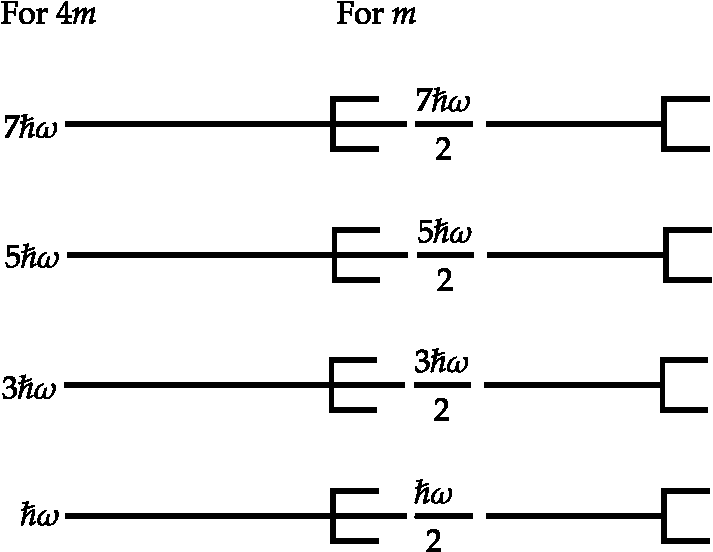
\includegraphics[height=4.5cm,width=6cm]{Net-June-20-32}
	\end{figure}
	 \begin{tasks}(2)
		\task[\text{a.}] $2\left(\frac{\hbar \omega}{2}\right)+2\left(\frac{3 \hbar \omega}{2}\right)=4 \hbar \omega$
		\task[\text{b.}]$2(\hbar \omega)+2(3 \hbar \omega)=8 \hbar \omega$
		\task[\text{c.}]$\frac{\hbar \omega}{2}+2(\hbar \omega)+3 \hbar \omega=\frac{11}{2} \hbar \omega=5.5 \hbar \omega$
		\task[\text{d.}] $2\left(\frac{\hbar \omega}{2}\right)+2(\hbar \omega)=3 \hbar \omega$
	\end{tasks}
$3 \hbar \omega$ is lowest among all\\
		So the correct answer is \textbf{Option (d)}
\end{answer}
\item  Falling drops of rain break up and coalesce with each other and finally achieve an approximately spherical shape in the steady state. The radius of such a drop scales with the surface tension $\sigma$ as
	 \begin{tasks}(4)
		\task[\textbf{a.}]$1 / \sqrt{\sigma}$
		\task[\textbf{b.}] $\sqrt{\sigma}$
		\task[\textbf{c.}]$\sigma$
		\task[\textbf{d.}] $\sigma^{2}$
	\end{tasks}
\begin{answer}
	\begin{align*}
\text{ Work done while combining }W&=\sigma \times\text{ change in area }=\sigma \times\left(4 \pi R^{2}-n 4 \pi r^{2}\right)\\
	\text{Taking small $r$ negligible: }W&=\sigma \times 4 \pi R^{2} \Rightarrow R \propto \frac{1}{\sqrt{\sigma}}
	\end{align*}
		So the correct answer is \textbf{Option (a)}
\end{answer}
\item  The velocity $v(x)$ of a particle moving in one dimension is given by $v(x)=v_{0} \sin \left(\frac{\pi x}{x_{0}}\right)$, where $v_{0}$ and $x_{0}$ are positive constants of appropriate dimensions. If the particle is initially at $x / x_{0}=\epsilon$, where $|\in| \ll 1$, then, in the long time, it
	 \begin{tasks}(1)
		\task[\textbf{a.}] Executes an oscillatory motion around $x=0$
		\task[\textbf{b.}]Tends towards $x=0$
		\task[\textbf{c.}] Tends towards $x=x_{0}$
		\task[\textbf{d.}] Executes an oscillatory motion around $x=x_{0}$
	\end{tasks}
\begin{answer}
	\begin{align*}
	v(x)&=v_{0} \sin \left(\frac{\pi x}{x_{0}}\right) \Rightarrow a(x)=v_{0} \cos \left(\frac{\pi x}{x_{0}}\right) \frac{\pi}{x_{0}} \cdot \frac{d x}{d t}=v_{0} \cos \left(\frac{\pi x}{x_{0}}\right) \frac{\pi}{x_{0}} \cdot v_{0} \sin \left(\frac{\pi x}{x_{0}}\right)\\
	a(x)&=\frac{\pi v_{0}^{2}}{2 x_{0}} \sin \left(\frac{2 \pi x}{x_{0}}\right) \Rightarrow a(x) \simeq \frac{\pi v_{0}^{2}}{2 x_{0}}\left(\frac{2 \pi x}{x_{0}}\right)=\frac{\pi^{2} v_{0}^{2}}{x_{0}^{2}} x\\
\text{	So motion }&\text{is not oscillatory.}\\
	\frac{d^{2} x}{d t^{2}}-k^{2} x&=0 \Rightarrow x=A e^{k t}+B e^{-k t} \text { where } k=\frac{\pi v_{0}}{x_{0}}\\
\intertext{	As $t \rightarrow \infty, x=A e^{k t}$ if we assume $k$ small and $t$ is large we can assume $x$ is some fixed quantity So}
	\end{align*}
		So the correct answer is \textbf{Option (c)}
\end{answer}
\item  A pendulum executes small oscillations between angles $+\theta_{0}$ and $-\theta_{0}$. If $\tau(\theta) d \theta$ is the time spent between $\theta$ and $\theta+d \theta$, then $\tau(\theta)$ is best represented by
 \begin{tasks}(2)
	\task[\textbf{a.}]
	\begin{figure}[H]
		\centering
		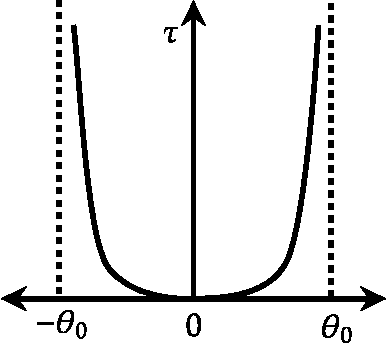
\includegraphics[height=3.5cm,width=4cm]{Net-June-20-33}
	\end{figure}
	\task[\textbf{b.}]
	\begin{figure}[H]
		\centering
		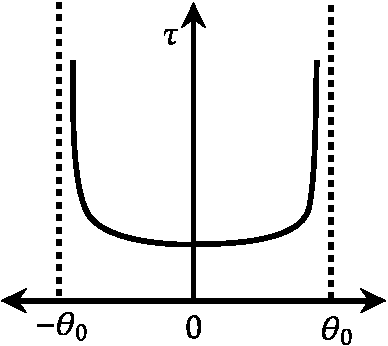
\includegraphics[height=3.5cm,width=4cm]{Net-June-20-34}
	\end{figure}
	\task[\textbf{c.}]
	\begin{figure}[H]
		\centering
		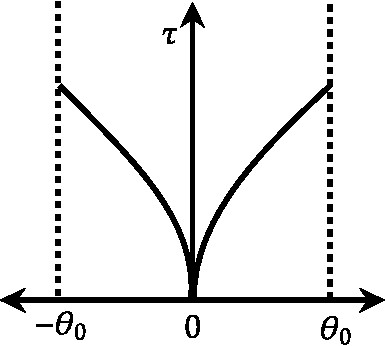
\includegraphics[height=3.5cm,width=4cm]{Net-June-20-35}
	\end{figure}
	\task[\textbf{d.}] 
	\begin{figure}[H]
		\centering
		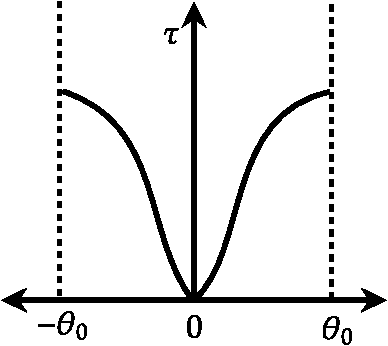
\includegraphics[height=3.5cm,width=4cm]{Net-June-20-36}
	\end{figure}
\end{tasks}
\begin{answer}
	So the correct answer is \textbf{Option (b)}
\end{answer}
\item Consider a particle with total energy $E$ moving in one dimension in a potential $V(x)$ as shown in the figure below
\begin{figure}[H]
	\centering
	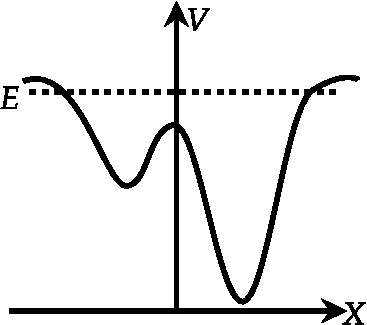
\includegraphics[height=2.5cm,width=3cm]{Net-June-20-37}
\end{figure}
Which of the following figures best represents the orbit of the particle in the phase space?
	 \begin{tasks}(2)
		\task[\textbf{a.}]
		\begin{figure}[H]
			\centering
			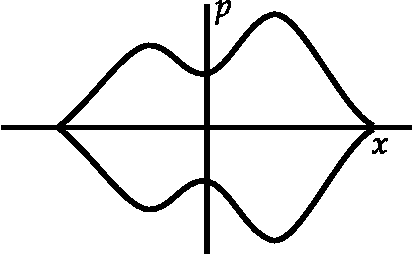
\includegraphics[height=2cm,width=3cm]{Net-June-20-38}
		\end{figure}
		\task[\textbf{b.}]
		\begin{figure}[H]
			\centering
			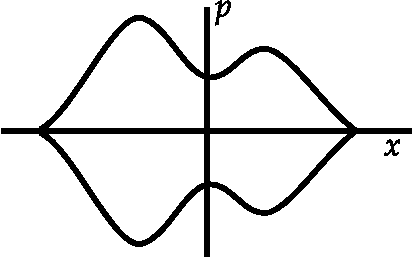
\includegraphics[height=2cm,width=3cm]{Net-June-20-39}
		\end{figure}
		\task[\textbf{c.}]
		\begin{figure}[H]
			\centering
			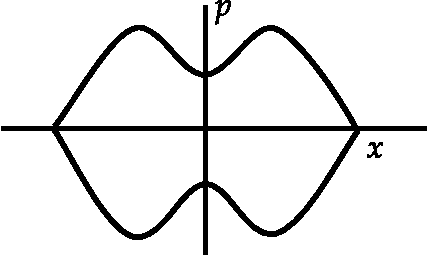
\includegraphics[height=2cm,width=3cm]{Net-June-20-40}
		\end{figure}
		\task[\textbf{d.}] 
		\begin{figure}[H]
			\centering
			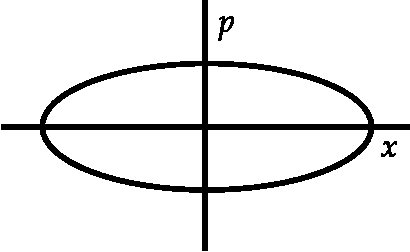
\includegraphics[height=2cm,width=3cm]{Net-June-20-41}
		\end{figure}
	\end{tasks}
\begin{answer}
	\begin{align*}
	\text { Use concept } T&=E-V \text { where } T \text { is kinetic energy } E \text { is total energy and } V \text { is potential energy. }
	\end{align*}
	So the correct answer is \textbf{Option (a)}
\end{answer}
\item The energy density $I$ of a black body radiation at temperature $T$ is given by the Planck's distribution function $I(v, T)=\frac{8 \pi v^{2}}{c^{3}} \frac{h v}{\left(e^{\frac{h v}{k_{B} T}}-1\right)}$, where $v$ is the frequency. The function $I(v, T)$ for two different temperatures $T_{1}$ and $T_{2}$ are shown below.
\begin{figure}[H]
	\centering
	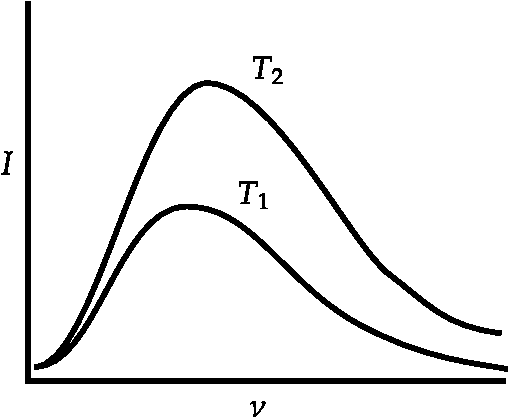
\includegraphics[height=3cm,width=4cm]{Net-June-20-42}
\end{figure}
 If the two curves coincide when $I(v, T) v^{a}$ is plotted against $v^{b} / T$, then the values of $a$ and $b$ are, respectively,
 \begin{tasks}(4)
	\task[\textbf{a.}] 2 and 1
	\task[\textbf{b.}]$-2$ and 2
	\task[\textbf{c.}]3 and $-1$
	\task[\textbf{d.}] $-3$ and 1
\end{tasks}
\begin{answer}
	\begin{align*}
	I&=\frac{8 \pi v^{3}}{c^{3}} \frac{h}{\left(\frac{h v}{e^{k_{B} T}}-1\right)} \Rightarrow y=I v^{a}=\frac{8 \pi v^{a+3}}{c^{3}} \frac{h}{\left(\frac{h v}{e^{k_{B} T}} v^{b} v^{-b}-1\right)}\\
	\text{Let }x&=v^{b} / T \Rightarrow y=\frac{8 \pi h}{c^{3}} \frac{v^{a+3}}{\left(e^{\frac{h v^{-b+1}}{k_{B}} x}-1\right)}\\
	\text{For, }a&=-3, b=1 ; \quad y=\alpha \frac{1}{\left(e^{\beta x}-1\right)}\text{Both graph are now same}
	\end{align*}
	So the correct answer is \textbf{Option (d)}
\end{answer}
\item For an ideal gas consisting of $N$ distinguishable particles in a volume $V$, the probability of finding exactly 2 particles in a volume $\delta V \ll V$, in the limit $N, V \rightarrow \infty$, is
 \begin{tasks}(2)
	\task[\textbf{a.}] $2 N \delta V / V$
	\task[\textbf{b.}]$(N \delta V / V)^{2}$
	\task[\textbf{c.}]$\frac{(N \delta V)^{2}}{2 V^{2}} e^{-N o V / V}$
	\task[\textbf{d.}]  $\left(\frac{\delta V}{V}\right)^{2} e^{-N o V / V}$
\end{tasks}
\begin{answer}$\left. \right. $
	\begin{figure}[H]
		\centering
		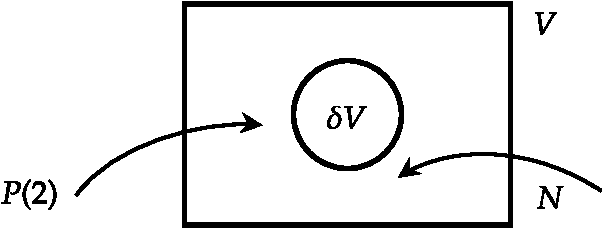
\includegraphics[height=2cm,width=5cm]{Net-June-20-43}
	\end{figure}
	\begin{align*}
	\text{We can use poisons here }f(x)&=\frac{\mu^{x}}{x !} e^{-\mu}\quad
\text{	where }\mu=N\left(\frac{\delta V}{V}\right)\\
f(2)&=\frac{\left[N\left(\frac{\delta V}{V}\right)\right]^{2}}{2 !} \cdot e^{-N\left(\frac{\delta V}{V}\right)}=\frac{(N \delta V)^{2}}{2 V^{2}} e^{-N\left(\frac{\delta V}{V}\right)}
	\end{align*}
		So the correct answer is \textbf{Option (c)}
\end{answer}
\item The Hamiltonian of a system of 3 spins is $H=J\left(S_{1} S_{2}+S_{2} S_{3}\right)$, where $S_{i}=\pm 1$ for $i=1,2,3$. Its canonical partition function, at temperature $T$, is
 \begin{tasks}(2)
	\task[\textbf{a.}]$2\left(2 \sinh \frac{J}{k_{B} T}\right)^{2}$
	\task[\textbf{b.}]$2\left(2 \cosh \frac{J}{k_{B} T}\right)^{2}$
	\task[\textbf{c.}]$2\left(2 \cosh \frac{J}{k_{B} T}\right)$
	\task[\textbf{d.}] $2\left(2 \cosh \frac{J}{k_{B} T}\right)^{3}$
\end{tasks}
\begin{answer}
	\begin{align*}
	\begin{array}{|c|c|c|c|}
	\hline S_{1} & S_{2} & S_{3} & H \\
	\hline 1 & 1 & 1 & 2 \mathrm{~J} \\
	\hline 1 & 1 & -1 & 0 \\
	\hline 1 & -1 & 1 & 0 \\
	\hline 1 & -1 & -1 & -2 \mathrm{~J} \\
	\hline-1 & 1 & 1 & 0 \\
	\hline-1 & 1 & -1 & -2 \mathrm{~J} \\
	\hline-1 & -1 & 1 & 0 \\
	\hline-1 & -1 & -1 & 2 \mathrm{~J} \\
	\hline
	\end{array}\\\\
	\text{Number of states }&2^{3}=8\\
	H&=J\left(S_{1} S_{2}+S_{2} S_{3}\right) \\
	Z&=2 e^{-\beta 2 J}+2 e^{\beta 2 J}+4=2\left[e^{\beta 2 J}+e^{-\beta 2 J}\right]+4=2\left(\left[e^{\beta J}+e^{-\beta J}\right]^{2}-2\right)+4 \\
	\Rightarrow Z&=2\left(\frac{2\left(e^{\beta J}+e^{-\beta J}\right)}{2}\right)^{2}=2\left(2 \cosh \frac{J}{k_{B} T}\right)^{2}
	\end{align*}
	So the correct answer is \textbf{Option (b)}
\end{answer}
\item  A certain two-dimensional solid crystallises to a square monoatomic lattice with lattice constant $a$. Each atom can contribute an integer number of free conduction electrons. The minimum number of electrons each atom must contribute such that the free electron Fermi circle at zero temperature encloses the first Brillouin zone completely, is
 \begin{tasks}(4)
	\task[\textbf{a.}]3
	\task[\textbf{b.}]1
	\task[\textbf{c.}]4
	\task[\textbf{d.}]2
\end{tasks}
\begin{answer}
	Brillouin zone of a square lattice of lattice constant ' $a$ ' is also a square as shown below
	\begin{figure}[H]
		\centering
		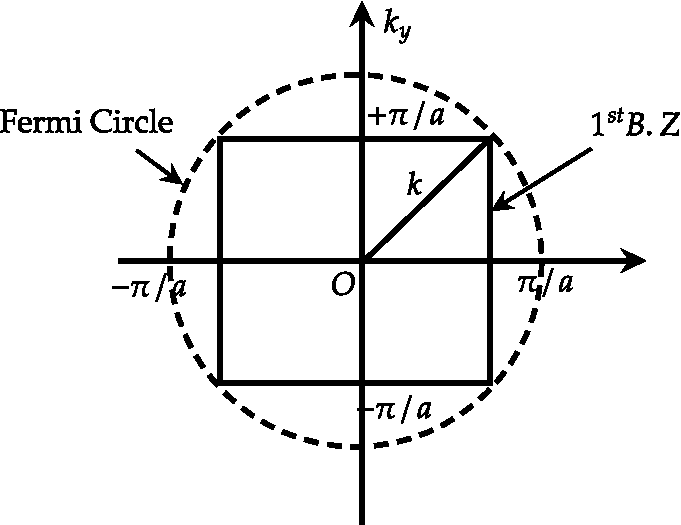
\includegraphics[height=5cm,width=6.7cm]{Net-June-20-44}
	\end{figure}
	The radius of the Fermi circle in two-dimension is
	\begin{align*}
	k_{F}&=(2 \pi n)^{1 / 2}=\left(2 \pi \frac{N}{a^{2}}\right)^{1 / 2}\\
\text{	The fermi circle }&\text{will enclose the $1^{\text {st }}$ B.Z completely}\\
	\text{If, }k_{F}&=k=\sqrt{2} \frac{\pi}{a}\\
	\therefore\left(2 \pi \frac{N}{a^{2}}\right)^{1 / 2}&=\frac{\sqrt{2} \pi}{a} \\
	\Rightarrow \frac{2 \pi N}{a^{2}}&=2 \frac{\pi^{2}}{a^{2}} \Rightarrow N=\pi=3.14\\
\intertext{	Since $N$ should be integer, therefore minimum number of electrons $(N)$ is 4}
	N&=4
	\end{align*}
		So the correct answer is \textbf{Option (c)}
\end{answer}
\item A tight binding model of electrons in one dimension has the dispersion relation $\varepsilon(k)=-2 t(1-\cos k a)$, where $t>0, a$ is the lattice constant and $-\frac{\pi}{a}<k<\frac{\pi}{a}$. Which of the following figures best represents the density of states over the range $\frac{\pi}{2 a} \leq k<\frac{\pi}{a}$ ?
 \begin{tasks}(2)
	\task[\textbf{a.}]
	\begin{figure}[H]
		\centering
		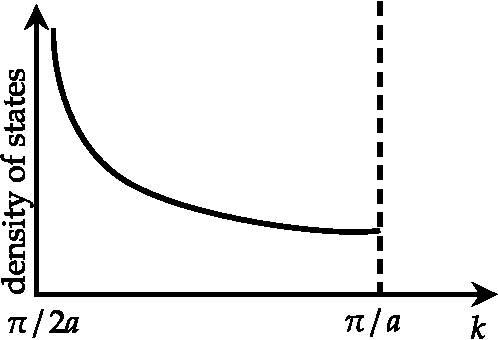
\includegraphics[height=3cm,width=4.2cm]{Net-June-20-45}
	\end{figure}
	\task[\textbf{b.}]
	\begin{figure}[H]
		\centering
		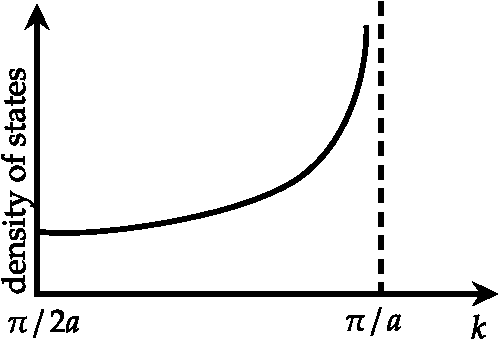
\includegraphics[height=3cm,width=4cm]{Net-June-20-46}
	\end{figure}
	\task[\textbf{c.}]
	\begin{figure}[H]
		\centering
		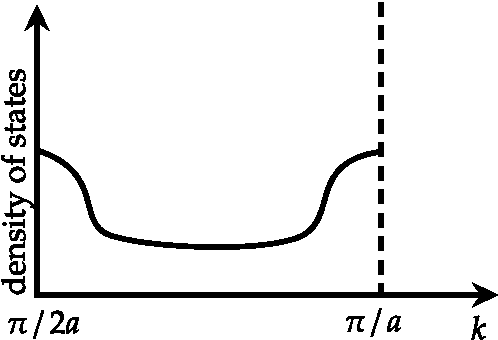
\includegraphics[height=3cm,width=4cm]{Net-June-20-47}
	\end{figure}
	\task[\textbf{d.}] 
	\begin{figure}[H]
		\centering
		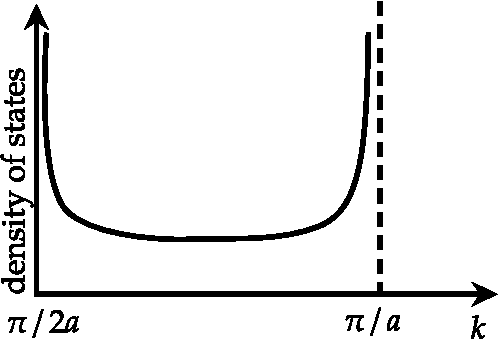
\includegraphics[height=3cm,width=4cm]{Net-June-20-48}
	\end{figure}
\end{tasks}
\begin{answer}
	\begin{align*}
	\varepsilon(k)&=-2 t(1-\cos k a) \Rightarrow d \varepsilon(k)=-2 t a \sin (k a) d k\\
	\text{Now, }g(k) d k&=\frac{L}{\pi} d k \Rightarrow g(\varepsilon) d \varepsilon=\frac{L}{\pi} \cdot \frac{d \varepsilon(k)}{-2 \operatorname{ta} \sin (k a)}\\
\text{	Density of state is } \rho(\varepsilon)&=\frac{g(\varepsilon) d \varepsilon}{d \varepsilon}=\frac{L}{-2 \pi t a} \cdot \frac{1}{\sin (k a)}\\
\text{at, }k&=\frac{\pi}{2 a}: \quad \rho(\varepsilon)=\frac{2}{2 \pi t a} \cdot \frac{1}{\sin \left(\frac{\pi}{2 a} \times a\right)}=\frac{L}{2 \pi t a}\\
\text{at }k&=\frac{\pi}{a}: \quad \rho(\varepsilon)=\frac{L}{2 \pi t a} \cdot \frac{1}{\sin \left(\frac{\pi}{a} \times a\right)}=\infty\\
\text { Thus, variation of } &\rho(\varepsilon) \text { vs } k \text { is }
	\end{align*}
	\begin{figure}[H]
		\centering
		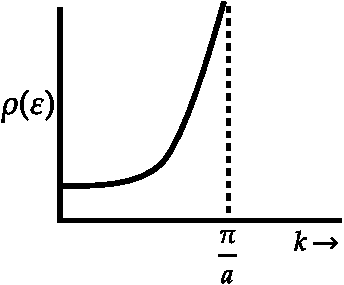
\includegraphics[height=3.5cm,width=4cm]{Net-June-20-49}
	\end{figure}
		So the correct answer is \textbf{Option (b)}
\end{answer}
\item A lattice is defined by the unit vectors $\vec{a}_{1}=a \hat{i}, \vec{a}_{2}=-\frac{a}{2} \hat{i}+\frac{a \sqrt{3}}{2} \hat{j}$ and $\vec{a}_{3}=a \hat{k}$, where $a>0$ is a constant. The spacing between the (100) planes of the lattice is
 \begin{tasks}(4)
	\task[\textbf{a.}] $\sqrt{3} a / 2$
	\task[\textbf{b.}]$a / 2$
	\task[\textbf{c.}] $a$
	\task[\textbf{d.}] $\sqrt{2} a$
\end{tasks}
\begin{answer}
	\begin{align*}
	\text{Interplanar  }&\text{spacing for Hexagonal lattice is}\\
	\frac{1}{d^{2}}&=\frac{4}{3}\left(\frac{h^{2}+h k+k^{2}}{a^{2}}\right)+\frac{l^{2}}{c^{2}}\\
\text{	Here }|a|&=\left|a_{1}\right|=a, \quad|b|=\left|a_{2}\right|=a\text{ and }|c|=\left|a_{3}\right|=a\text{ For $(100)$ plane}\\
	\frac{1}{d^{2}}&=\frac{4}{3}\left(\frac{1+0+0}{a^{2}}\right)+\frac{0}{c^{2}} \Rightarrow \frac{1}{d^{2}}=\frac{4}{3 a} \Rightarrow d=\frac{\sqrt{3}}{2} a
	\end{align*}
	So the correct answer is \textbf{Option (a)}
\end{answer}
\item  A spacecraft of mass $m=1000 \mathrm{~kg}$ has a fully reflecting sail that is oriented perpendicular to the direction of the sun. The sun radiates $10^{26} \mathrm{~W}$ and has a mass $M=10^{30} \mathrm{~kg}$. Ignoring the effect of the planets, for the gravitational pull of the sun to balance the radiation pressure on the sail, the area of the sail will be
 \begin{tasks}(4)
	\task[\textbf{a.}]$10^{2} \mathrm{~m}^{2}$
	\task[\textbf{b.}]$10^{4} \mathrm{~m}^{2}$
	\task[\textbf{c.}]$10^{8} \mathrm{~m}^{2}$
	\task[\textbf{d.}] $10^{6} \mathrm{~m}^{2}$
\end{tasks}
\begin{answer}$\left. \right. $
	\begin{figure}[H]
		\centering
		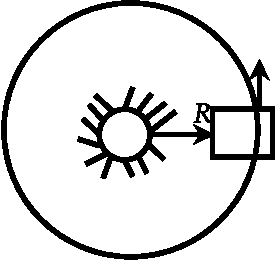
\includegraphics[height=2.5cm,width=2.8cm]{Net-June-20-50}
	\end{figure}
	\begin{align*}
	m&=10^{3} \mathrm{~kg}\\
	M&=10^{30} \mathrm{~kg} \\
	P&=10^{26} \mathrm{~W}\\
	\text{Radiation pressure  }&\text{for fully reflecting Surface}=\frac{2 I}{c}\\
	I=\text { Intensity }&=\frac{\text { Power }}{\text { Area }}=\frac{P}{4 \pi R^{2}}\\
	\text{Radiation Pressure }&=\frac{2 P}{4 \pi R^{2} c}\\
	\text{Gravitational pull }&=\frac{G M m}{R^{2}}\\
	\text{Force on sail }&=\text{ Radiation Press $\times$ Area of sail }=\frac{2 P}{4 \pi R^{2} c} \times A\\
	\frac{P}{2 \pi R^{2} c} \times A&=\frac{G M m}{R^{2}} \Rightarrow A=\frac{G M m \times 2 \pi c}{P} \Rightarrow A\\&=\frac{6.67 \times 10^{-11} \times 10^{30} \times 10^{3} \times 2 \pi \times 3 \times 10^{8}}{10^{26}} \\
	\Rightarrow A&=6.67 \times 6 \pi \times 10^{4}=125.72 \times 10^{4}=1.25 \times 10^{6}
	\end{align*}
		So the correct answer is \textbf{Option (d)}
\end{answer}
\item The electric field due to a uniformly charged infinite line along the $z$-axis, as observed in the rest frame $S$ of the line charge, is $\vec{E}(\vec{r})=\frac{\lambda}{2 \pi \epsilon_{0}} \frac{x \hat{i}+y \hat{j}}{\left(x^{2}+y^{2}\right)}$. In a frame $M$ moving with a constant speed $v$ with respect to $S$ along the $z$ - direction, the electric field $\vec{E}^{\prime}$ is (in the following $\beta=v / c$ and $\gamma=1 / \sqrt{1-\beta^{2}}$ )
 \begin{tasks}(2)
	\task[\textbf{a.}]$E_{x}^{\prime}=E_{x}$ and $E_{y}^{\prime}=E_{y}$
	\task[\textbf{b.}]$E_{x}^{\prime}=\beta \gamma E_{x}$ and $E_{y}^{\prime}=\beta \gamma E_{y}$
	\task[\textbf{c.}]$E_{x}^{\prime}=E_{x} / \gamma$ and $E_{y}^{\prime}=E_{y} / \gamma$
	\task[\textbf{d.}]  $E_{x}^{\prime}=\gamma E_{x}$ and $E_{y}^{\prime}=\gamma E_{y}$
\end{tasks}
\begin{answer}
	\begin{align*}
	M \text { is moving in }& z \text {-direction }\\
	E_{z}^{\prime}=E_{z}, E_{x}^{\prime}&=\gamma\left(E_{x}-v B_{y}\right), E_{y}^{\prime}=\gamma\left(E_{y}+v B_{x}\right)\text{ where }B_{x}=0, B_{y}=0\\
	\text{ Thus }E_{x}^{\prime}&=\gamma E_{x}\text{ and } E_{y}^{\prime}=\gamma E_{y}.
	\end{align*}
	So the correct answer is \textbf{Option (d)}
\end{answer}
\item A parallel plate capacitor with rectangular plates of length $l$, breadth $b$ and plate separation $d$, is held vertically on the surface of a dielectric liquid of dielectric constant $\kappa$ and density $\rho$ as shown in the figure. The length and breadth are large enough for edge effects to be neglected.
\begin{figure}[H]
	\centering
	\includegraphics[height=3cm,width=3cm]{Net-June-20-51}
\end{figure}
The plates of the capacitor are kept at a constant voltage difference $V$. Ignoring effects of surface tension, the height $h$ upto which the liquid level rises inside the capacitor, is
 \begin{tasks}(4)
	\task[\textbf{a.}]$\frac{V^{2} \varepsilon_{0}(\kappa-1)}{\rho g b d}$
	\task[\textbf{b.}]$\frac{V^{2} \varepsilon_{0}(\kappa-1)}{2 \rho g b^{2}}$
	\task[\textbf{c.}]$\frac{V^{2} \varepsilon_{0}(\kappa-1)}{2 \rho g d^{2}}$
	\task[\textbf{d.}] $\frac{V^{2} \varepsilon_{0}(\kappa-1)}{\rho g d^{2}}$
\end{tasks}
\begin{answer}
	\begin{align*}
	\text { Upward force on dielectric } F&=\frac{\varepsilon_{0} b V^{2}}{2 d}(\kappa-1)\\
\text{	If liquid rises to height $h$, then}\\
	\frac{\varepsilon_{0} b V^{2}(\kappa-1)}{2 d}&=(h b d) \rho g \Rightarrow h=\frac{\varepsilon_{0} V^{2}(\kappa-1)}{2 d^{2} \rho g}
	\end{align*}
	So the correct answer is \textbf{Option (c)}
\end{answer}
\item  Using the following values of $x$ and $f(x)$\\\\
\begin{tabular}{|c|c|c|c|c|}
	\hline$x$ & 0 & $0.5$ & $1.0$ & $1.5$ \\
	\hline$f(x)$ & 1 & $a$ & 0 & $-5 / 4$ \\
	\hline
\end{tabular}\\\\
the integral $I=\int_{0}^{1.5} f(x) d x$, evaluated by the Trapezoidal rule, is $5 / 16$. The value of $a$ is
 \begin{tasks}(4)
	\task[\textbf{a.}]$3 / 4$
	\task[\textbf{b.}]$3 / 2$
	\task[\textbf{c.}] $7 / 4$
	\task[\textbf{d.}] 19/24
\end{tasks}
\begin{answer}
	\begin{align*}
	I&=\frac{h}{2}\left[y_{0}+y_{n}+2\left(y_{1}+y_{2}+\cdots\right)\right]=\frac{1}{4}\left[1-\frac{5}{4}+2(a+0)\right]=\frac{5}{16}\\
	&\Rightarrow 1-\frac{5}{4}+2 a=\frac{5}{4} \\
	&\Rightarrow 2 a=\frac{10}{4}-1 \Rightarrow 2 a=\frac{6}{4} \Rightarrow a=\frac{3}{4}
	\end{align*}
		So the correct answer is \textbf{Option (a)}
\end{answer}
\item The Green's function for the differential equation $\frac{d^{2} x}{d t^{2}}+x=f(t)$, satisfying the initial conditions $x(0)=\frac{d x}{d t}(0)=0$ is
$$
G(t, \tau)=\left\{\begin{array}{llc}
0 & \text { for } & 0<t<\tau \\
\sin (t-\tau) & \text { for } & t>\tau
\end{array}\right.
$$
The solution of the differential equation when the source $f(t)=\theta(t)$ (the Heaviside step function) is
 \begin{tasks}(4)
	\task[\textbf{a.}]$\sin t$
	\task[\textbf{b.}]$1-\sin t$
	\task[\textbf{c.}]$1-\cos t$
	\task[\textbf{d.}]$\cos ^{2} t-1$ 
\end{tasks}
\begin{answer}
	\begin{align*}
	\frac{d^{2} x}{d t^{2}}+x&=f(t) \text { and } \quad x(0)=\dot{x}(0)=0\\
	G(t, \tau)&= \begin{cases}0, & 0<t<\tau \\
	\sin (t-\tau), \quad t>\tau\end{cases} \\
	x(t)&=\int_{0}^{\infty} G(t, \tau) f(\tau) d \tau \\
	\Rightarrow x(t)&=\int_{0}^{t} \sin (t-\tau) f(\tau) d \tau=\int_{0}^{t} \sin (t-\tau) d \tau=+\left.\cos (t-\tau)\right|_{0} ^{t}=1-\cos t
	\end{align*}
	So the correct answer is \textbf{Option (c)}
\end{answer}
		So the correct answer is \textbf{Option (c)}
\item The solution of the differential equation $\left(\frac{d y}{d x}\right)^{2}-\frac{d^{2} y}{d x^{2}}=e^{y}$, with the boundary conditions $y(0)=0$ and $y^{\prime}(0)=-1$, is
 \begin{tasks}(2)
	\task[\textbf{a.}]$-\ln \left(\frac{x^{2}}{2}+x+1\right)$
	\task[\textbf{b.}]$-x \ln (e+x)$
	\task[\textbf{c.}]$-x e^{-x^{2}}$
	\task[\textbf{d.}] $-x(x+1) e^{-x}$
\end{tasks}
\begin{answer}
	\begin{align*}
	\left(\frac{d y}{d x}\right)^{2}-\frac{d^{2} y}{d x^{2}}&=e^{y} \quad \text { put } y=\ln p\\
	\frac{d y}{d x}=\frac{1}{p} \frac{d p}{d x} &\Rightarrow \frac{d^{2} y}{d x^{2}}=\frac{d}{d x}\left(\frac{1}{p} \frac{d p}{d x}\right)=\frac{1}{p} \frac{d^{2} p}{d x^{2}}-\frac{1}{p^{2}}\left(\frac{d p}{d x}\right)^{2}\\
	\text { Thus }\left(\frac{1}{p} \frac{d p}{d x}\right)^{2}&-\frac{1}{p} \frac{d^{2} p}{d x^{2}}+\frac{1}{p^{2}}\left(\frac{d p}{d x}\right)^{2}=p \\
	\frac{2}{p^{2}}\left(\frac{d p}{d x}\right)^{2}-\frac{1}{p} \frac{d^{2} p}{d x^{2}}&=p \Rightarrow \frac{2}{p^{3}}\left(\frac{d p}{d x}\right)^{2}-\frac{1}{p^{2}} \frac{d^{2} p}{d x^{2}}=1 \Rightarrow \frac{1}{p^{2}} \frac{d^{2} p}{d x^{2}}-\frac{2}{p^{3}}\left(\frac{d p}{d x}\right)^{2}=-1 \\
	\Rightarrow \frac{d}{d x}\left(\frac{1}{p^{2}} \frac{d p}{d x}\right)&=-1\\
	\text { Let } \frac{1}{p^{2}} \frac{d p}{d x}&=z \Rightarrow \frac{d z}{d x}=-1 \Rightarrow z=-x+c\\
	\text { Thus } \frac{1}{p^{2}} \frac{d p}{d x}&=-x+c \Rightarrow \int \frac{d p}{p^{2}}=\int(-x+c) d x\\
	-\frac{1}{p}&=-\frac{x^{2}}{2}+c x+d \Rightarrow p=\frac{1}{\frac{x^{2}}{2}-c x-d} \\
	y&=\ln p=\ln \left(\frac{1}{\frac{x^{2}}{2}-c x-d}\right)=\ln \left(\frac{x^{2}}{2}-c x-d\right) \\
	y(0)&=0 \Rightarrow y(0)=-\ln (-d) \Rightarrow d=-1\\
	y&=-\ln \left(\frac{x^{2}}{2}-c x+1\right) \\
	y^{\prime}(x)&=-\frac{1}{\left(\frac{x^{2}}{2}-c x+1\right)}(x-c), \quad y^{\prime}(0)=-1 \Rightarrow-\frac{(-c)}{1}=c=-1, \quad y=-\ln \left(\frac{x^{2}}{2}+x+1\right)
	\end{align*}
	So the correct answer is \textbf{Option (a)}
\end{answer}
\item  If we take the nuclear spin $I$ into account, the total angular momentum is $\vec{F}=\vec{L}+\vec{S}+\vec{I}$, where $\vec{L}$ and $\vec{S}$ are the orbital and spin angular momenta of the electron. The Hamiltonian of the hydrogen atom is corrected by the additional interaction $\lambda \vec{I} \cdot(\vec{L}+\vec{S})$, where $\lambda>0$ is a constant. The total angular momentum quantum number $F$ of the $p$-orbital state with the lowest energy is
 \begin{tasks}(4)
	\task[\textbf{a.}]0
	\task[\textbf{b.}]1
	\task[\textbf{c.}]$1 / 2$
	\task[\textbf{d.}] $3 / 2$
\end{tasks}
\begin{answer}
	\begin{align*}
	\vec{F}&=\vec{L}+\vec{S}+\vec{I}=\vec{J}+\vec{I} ; \quad H=\lambda \vec{I} \cdot(\vec{L}+\vec{S})=\lambda \vec{I} \cdot \vec{J}\\
	\Rightarrow H&=\lambda \frac{F^{2}-I^{2}-J^{2}}{2} \quad \therefore \vec{F}=\vec{J}+\vec{I}\\
	F^{2}&=J^{2}+I^{2}+2 \vec{I} \cdot \vec{J}\\
	\text { For hydrogen atom, } &p \text {-orbital electron }\\
	L&=1, S=\frac{1}{2} \rightarrow J=\frac{1}{2}, \frac{3}{2}\\
	I&=\frac{1}{2}\qquad \begin{aligned}
	&J=\frac{1}{2} \rightarrow F=0,1 \\
	&J=\frac{3}{2} \rightarrow F=1,2
	\end{aligned}\\
	\Delta E&=\lambda \frac{F(F+1)-I(I+1)-J(J+1)}{2} \hbar^{2} \\
	\Delta E_{1}&\left(F=0, I=\frac{1}{2}, J=\frac{1}{2}\right) ; \quad \Delta E_{1}=\lambda \frac{0-\frac{3}{4}-\frac{3}{4}}{2} \hbar^{2}=-\frac{3}{4} \lambda \hbar^{2}\\
	\Delta E_{2}&\left(F=I, I=\frac{1}{2}, J=\frac{1}{2}\right) ; \quad \Delta E_{2}=\lambda \frac{2-\frac{3}{4}-\frac{3}{4}}{2} \hbar^{2}=\frac{1}{4} \lambda \hbar^{2} \\
	\Delta E_{3}&\left(F=1, I=\frac{1}{2}, J=\frac{3}{2}\right) ; \quad \Delta E_{3}=\lambda \frac{2-\frac{3}{4}-\frac{15}{4}}{2} \hbar^{2}=-\frac{5}{4} \lambda \hbar^{2}\\
	\Delta E_{4}&\left(F=2, I=\frac{1}{2}, J=\frac{3}{2}\right) ; \quad \Delta E_{4}=\lambda \frac{6-\frac{3}{4}-\frac{15}{4}}{2}=\frac{3}{4} \lambda \hbar^{2}
	\intertext{Out of these four possibilities lowest state is corresponding to following quantum number}
	F&=1, I=\frac{1}{2}, J=\frac{3}{2}, L=1, S=\frac{1}{2}
	\end{align*}
		So the correct answer is \textbf{Option (b)}
\end{answer}
\item  The absorption lines arising from pure rotational effects of $\mathrm{HCl}$ are observed at $83.03 \mathrm{~cm}^{-1}$, $103.73 \mathrm{~cm}^{-1}, 124.30 \mathrm{~cm}^{-1}, 145.03 \mathrm{~cm}^{-1}$ and $165.51 \mathrm{~cm}^{-1}$. The moment of inertia of the $\mathrm{HCl}$ molecule is (take $\frac{\hbar}{2 \pi c}=5.6 \times 10^{-44} \mathrm{~kg}-\mathrm{m}$ )
 \begin{tasks}(2)
	\task[\textbf{a.}] $1.1 \times 10^{-48} \mathrm{~kg}-\mathrm{m}^{2}$
	\task[\textbf{b.}]$2.8 \times 10^{-47} \mathrm{~kg}-\mathrm{m}^{2}$
	\task[\textbf{c.}]$2.8 \times 10^{-48} \mathrm{~kg}-\mathrm{m}^{2}$
	\task[\textbf{d.}] $1.1 \times 10^{-42} \mathrm{~kg}-\mathrm{m}^{2}$
\end{tasks}
\begin{answer}
	\begin{align*}
	2 B&=103.73-83.03=20.70 \mathrm{~cm}^{-1} \quad \Rightarrow 2 B=124.30-103.73=20.57 \mathrm{~cm}^{-1}\\
	\Rightarrow 2 B&=145.03-124.30=20.73 \mathrm{~cm}^{-1}\\
\text{	Average value }2 B&=\frac{62.00}{3}=20.67 \mathrm{~cm}^{-1} \Rightarrow B=10.33 \mathrm{~cm}^{-1}=1033 \mathrm{~m}^{-1}\\
	I&=\frac{h}{8 \pi^{2} B c}=\frac{27.99 \times 10^{-45}}{B} \mathrm{~kg}-\mathrm{m}^{2}=\frac{27.99 \times 10^{-45}}{1033}=2.7 \times 10^{-47} \mathrm{~kg}-\mathrm{m}^{2}\\
	\frac{h}{8 \pi^{2} c}&=27.99 \times 10^{-45}\text{ in SI unit.}
	\end{align*}
		So the correct answer is \textbf{Option (b)}
\end{answer}
\item  The energies of the 3 lowest states of an atom are $E_{0}=-14 \mathrm{eV}, E_{1}=-9 \mathrm{eV}$ and $E_{2}=-7 \mathrm{eV}$. The Einstein coefficients are $A_{10}=3 \times 10^{8} \mathrm{~s}^{-1}, A_{20}=1.2 \times 10^{8} \mathrm{~s}^{-1}$ and $A_{21}=8 \times 10^{7} \mathrm{~s}^{-1}$. If a large number of atoms are in the energy level $E_{2}$, the mean radiative lifetime of this excited state is
 \begin{tasks}(2)
	\task[\textbf{a.}] $8.3 \times 10^{-9} \mathrm{~s}$
	\task[\textbf{b.}]$1 \times 10^{-8} s$
	\task[\textbf{c.}]$0.5 \times 10^{-8} \mathrm{~s}$
	\task[\textbf{d.}]$1.2 \times 10^{-8} s$ 
\end{tasks}
\begin{answer}
	\begin{align*}
	\text { Rate of }&\text{spontaneous decay from } E_{2} \text { state }\\
	&=\left(A_{20}+A_{21}\right) N_{1}=A_{2} N_{1} \\
	A_{2}&=A_{20}+A_{21}=\left(1.2 \times 10^{8}+0.8 \times 10^{8}\right) \mathrm{s}^{-1}=2.0 \times 10^{8} \mathrm{~s}^{-}\\
	\therefore &\text{ Mean radiative life time }\\
	\tau_{2}&=\frac{1}{A_{2}}=\frac{1}{2.0 \times 10^{8}}=0.5 \times 10^{-8} \mathrm{~s}
	\end{align*}
		So the correct answer is \textbf{Option (c)}
\end{answer}
\item  Two voltmeters $A$ and $B$ with internal resistances $2 M \Omega$ and $0.1 k \Omega$ are used to measure the voltage drops $V_{A}$ and $V_{B}$, respectively, across the resistor $R$ in the circuit shown below.
\begin{figure}[H]
	\centering
	\includegraphics[height=3cm,width=7cm]{Net-June-20-52}
\end{figure}
The ratio $V_{A} / V_{B}$ is
 \begin{tasks}(4)
	\task[\textbf{a.}]$0.58$
	\task[\textbf{b.}] $1.73$
	\task[\textbf{c.}]1
	\task[\textbf{d.}] 2
\end{tasks}
\begin{answer}
	Let us draw Thevenin's equivalent across point ab:
	\begin{figure}[H]
		\centering
		\includegraphics[height=7cm,width=10cm]{Net-June-20-53}
	\end{figure}
Equivalent Circuit:
\begin{figure}[H]
	\centering
	\includegraphics[height=2.3cm,width=5cm]{Net-June-20-54}
\end{figure}
Voltmeter is connected across point ac in parallel.\\
Case A: Voltmeter internal resistance is $2 M \Omega$, so equivalent resistance across ac is
	\begin{align*}
	&=\frac{100 \Omega \times 2 M \Omega}{100 \Omega+2 M \Omega} \approx 100 \Omega \\
	\text{So }V_{A} &=\frac{100}{360} \times 12 V=\frac{10}{3} V
	\end{align*}
	Case B: Voltmeter internal resistance is $0.1 k \Omega=100 \Omega$, so equivalent resistance across ac is
	\begin{align*}
	&=\frac{100 \Omega \times 100 \Omega}{100 \Omega+100 \Omega}=50 \Omega\\
	\text { So } V_{B}&=\frac{50}{310} \times 12 V=\frac{600}{310} V=\frac{60}{31} V\\
	\Rightarrow \frac{V_{A}}{V_{B}}&=\frac{10 / 3}{60 / 31}=\frac{10}{60} \times \frac{31}{3}=1.72
	\end{align*}
	So the correct answer is \textbf{Option (b)}
\end{answer}
\item  The $I-V$ characteristics of the diode $D$ in the circuit below is given by
$$
I=I_{s}\left(e^{\frac{q V}{k_{B} T}}-1\right)
$$
where $I_{s}$ is the reverse saturation current, $V$ is the voltage across the diode and $T$ is the absolute temperature.\\
If the input voltage is $V_{\text {in }}$, then the output voltage $V_{\text {out }}$ is
 \begin{tasks}(2)
	\task[\textbf{a.}]$I_{S} R \ln \left(\frac{q V_{i n}}{k_{B} T}+1\right)$
	\task[\textbf{b.}]$\frac{1}{q} k_{B} T \ln \left(\frac{q\left(V_{i n}+I_{S} R\right)}{k_{B} T}\right)$
	\task[\textbf{c.}]$\frac{1}{q} k_{B} T \ln \left(\frac{V_{i n}}{I_{S} R}+1\right)$
	\task[\textbf{d.}] $-\frac{1}{q} k_{B} T \ln \left(\frac{V_{i n}}{I_{S} R}+1\right)$
\end{tasks}
\begin{answer}
	\begin{align*}
	\because I&=I_{R} \quad \Rightarrow I_{S}\left(e^{e V_{D} / k_{B} T}-1\right)=\frac{0-\left(-V_{i n}\right)}{R}\\
	\Rightarrow e^{e V_{D} / k_{B} T}-1&=+\frac{V_{i n}}{I_{S} R} \Rightarrow e^{e V_{D} / k_{B} T}=\frac{V_{i n}}{I_{S} R}+1 \Rightarrow V_{D}=\frac{k_{B} T}{e} \ln \left(\frac{V_{i n}}{I_{S} R}+1\right)
	\end{align*}
		So the correct answer is \textbf{Option (c)}
\end{answer}
\item A rod pivoted at one end is rotating clockwise 25 times a second in a plane. A video camera which records at a rate of 30 frames per second is used to film the motion. To someone watching the video, the apparent motion of the rod will seem to be
 \begin{tasks}(1)
	\task[\textbf{a.}] 10 rotations per second in the clockwise direction
	\task[\textbf{b.}]10 rotations per second in the anticlockwise direction
	\task[\textbf{c.}]5 rotations per second in the clockwise direction
	\task[\textbf{d.}] 5 rotations per second in the anticlockwise direction
\end{tasks}
\begin{answer}
		So the correct answer is \textbf{Option (d)}
\end{answer}
\item  In the circuit shown below, the gain of the op-amp in the middle of its bandwidth is $10^{5}$. A sinusoidal voltage with angular frequency $\omega=100 \mathrm{rad} / \mathrm{s}$ is applied to the input of the op--amp.
\begin{figure}[H]
	\centering
	\includegraphics[height=3.3cm,width=6cm]{Net-June-20-56}
\end{figure}
The phase difference between the input and the output voltage is
 \begin{tasks}(4)
	\task[\textbf{a.}]$5 \pi / 4$
	\task[\textbf{b.}]$3 \pi / 4$
	\task[\textbf{c.}]$\pi / 2$
	\task[\textbf{d.}]$\pi$ 
\end{tasks}
\begin{answer}
	\begin{align*}
	\frac{v_{0}}{v_{m}}&=\frac{-R_{2}}{R_{1}+X_{C}} \Rightarrow \frac{v_{0}}{v_{m}}=\frac{-4 \times 10^{3}}{2 \times 10^{3}+\frac{1}{j \times 100 \times 5 \times 10^{-6}}}=\frac{4}{2-2 j}\\&=-\frac{4}{\sqrt{4+4} e^{-j \pi / 4}}=-\sqrt{2} e^{j \pi / 4}\\
	\Rightarrow \frac{v_{0}}{v_{m}}&=\sqrt{2} e^{j \pi} e^{j \pi / 4}=\sqrt{2} e^{j 5 \pi / 4}\\
	&\Rightarrow \text { Input lags output by } \frac{5 \pi}{4}
	\end{align*}
	So the correct answer is \textbf{Option (a)}
\end{answer}
\item Charged pions $\pi^{-}$decay to muons $\mu^{-}$and anti-muon neutrinos $\vec{v}_{\mu} ; \pi^{-} \rightarrow \mu^{-}+\vec{v}_{\mu}$. Take the rest masses of a muon and a pion to be $105 \mathrm{MeV}$ and $140 \mathrm{MeV}$, respectively. The probability that the measurement of the muon spin along the direction of its momentum is positive, is closest to
 \begin{tasks}(4)
	\task[\textbf{a.}]$0.5$
	\task[\textbf{b.}]$0.75$
	\task[\textbf{c.}]1
	\task[\textbf{d.}] 0
\end{tasks}
\begin{answer}
		So the correct answer is \textbf{Option (c)}
\end{answer}
\item  The binding energy $B$ of a nucleus is approximated by the formula $B=a_{1} A-a_{2} A^{2 / 3}-a_{3} Z^{2} A^{-1 / 3}-a_{4}(A-2 Z)^{2} A^{-1}$, where $Z$ is the atomic number and $A$ is the mass number of the nucleus. If $\frac{a_{4}}{a_{2}} \simeq 30$. The atomic number $Z$ for naturally stable isobars (constant value of $A$ ) is
 \begin{tasks}(4)
	\task[\textbf{a.}]$\frac{30 A}{60+A^{2 / 3}}$
	\task[\textbf{b.}]$\frac{30 A}{30+A^{2 / 3}}$
	\task[\textbf{c.}]$\frac{60 A}{120+A^{2 / 3}}$
	\task[\textbf{d.}]  $\frac{120 A}{60+A^{2 / 3}}$
\end{tasks}
\begin{answer}
	\begin{align*}
	B&=a_{1} A-a_{2} A^{2 / 3}-a_{3} Z^{2} A^{-1 / 3}-a_{4}(A-2 Z)^{2} A^{-1}\\
	\text { For most isobar } \frac{\partial B}{\partial Z}&=0 \Rightarrow-\frac{a_{3}(2 Z)}{A^{1 / 3}}-\frac{a_{4} 2(A-2 Z)(-2)}{A}=0\\
	\Rightarrow a_{3} \frac{Z}{A^{1 / 3}}&=2 a_{4} \frac{A}{A}-4 a_{4} \frac{Z}{A} \\
	\Rightarrow \frac{Z}{A}\left(a_{3} A^{2 / 3}+4 a_{4}\right)&=2 a_{4} \Rightarrow Z=\frac{2 a_{4} A}{a_{3} A^{2 / 3}+4 a_{4}}=\frac{A}{2+\frac{a_{3}}{2 a_{4}} A^{2 / 3}}\\
	\Rightarrow Z&=\frac{A}{2+\frac{1}{60} A^{2 / 3}}=\frac{60 A}{120+A^{2 / 3}}
	\end{align*}
		So the correct answer is \textbf{Option (c)}
\end{answer}
\item  The magnetic moments of a proton and a neutron are $2.792 \mu_{N}$ and $-1.913 \mu_{N}$, where $\mu_{N}$ is the nucleon magnetic moment. The values of the magnetic moments of the mirror nuclei ${ }_{9}^{19} F_{10}$ and ${ }_{10}^{19} \mathrm{Ne}_{9}$, respectively, in the Shell model, are closest to
 \begin{tasks}(2)
	\task[\textbf{a.}]$23.652 \mu_{N}$ and $-18.873 \mu_{N}$
	\task[\textbf{b.}]$26.283 \mu_{N}$ and $-16.983 \mu_{N}$
	\task[\textbf{c.}]$-2.628 \mu_{N}$ and $1.887 \mu_{N}$
	\task[\textbf{d.}]  $2.628 \mu_{N}$ and $-1.887 \mu_{N}$
\end{tasks}
\begin{answer}
	\begin{align*}
	{ }_{9}^{19} F_{10}&: p(9): 1 s_{1 / 2}^{2} 1 p_{3 / 2}^{2} 1 p_{1 / 2}^{2} 1 d_{5 / 2}^{2}\\
	j&=\frac{5}{2}=2+\frac{1}{2}=l+\frac{1}{2}\\
	\left\langle\mu_{Z}\right\rangle_{F^{19}}&=\mu_{N}(i+2.29)=\mu_{N}(2.5+2.29)=4.79 \mu_{N} \\
	{ }_{10}^{19} N e_{9}&: N(9): 1 s_{1 / 2}^{2} 1 p_{3 / 2}^{4} 1 p_{1 / 2}^{2} 1 d_{5 / 2}^{1} \\
	j&=\frac{5}{2}=l+\frac{1}{2}\\
	\left\langle\mu_{z}\right\rangle_{N e^{19}}&=-1.91 \mu_{N}
	\end{align*}
		So the correct answer is \textbf{Option (d)}
\end{answer}








\end{enumerate}